% !TEX root = ./setup.tex

\section{Introduction}
Interactive museum exhibits create experiences that are more enjoyable and immersive. Visitors feel more engaged and can identify better with a museum's collection when they can interact with it. The Dutch Resistance Museum\footnote{Dutch Resistance Museum - Verzetsmuseum, \url{https://www.verzetsmuseum.org/museum/en/museum}, Accessed 08-02-2018} in Amsterdam is looking for ways to increase the interactivity and engagement between visitors and the twelve main dilemmas in their main exhibition. This paper proposes a solution where multiple exhibits are digitally augmented with screens and RFID readers that visitors can interact with by means of smart identity card replicas. In its premise, it lets visitors decide on a set of dilemmas that Dutch citizens faced during World War II (WWII) and afterwards, it shows the popularity of the visitor's choices and creates a personalized story out of their choices.\\

\noindent This research investigates the design and implementation of an interactive museum experience for the Dutch Resistance Museum, that highlights the dilemmas people faced during the occupation of the Netherlands between 1940-1945.\\

\noindent The design of \textit{Identification Rumble} as an interactive museum experience was the result of a collaboration between Master of Science (MSc) students from the University of Amsterdam (UvA), staff from the Dutch Resistance Museum and students from Media College Amsterdam. \\

\noindent Section \ref{sec:stakeholder} examines the expectations of the museum staff as well as key challenges within the project domain. Hereafter section \ref{relwork} offers a short review of related work. Section \ref{probmed} describes the problem statement and methodological approach underlying this research. Section \ref{intexper} provides an overview of the design process from concept to a final interaction journey proposal. Section \ref{systemdescription} presents a detailed description of the system. Finally section \ref{discussion} discusses feedback, limitations and provides a conclusion, recommendation and future work.


\subsection{Stakeholder} \label{sec:stakeholder}
From 1940 to 1945 the Netherlands were occupied by Nazi Germany. The Dutch Resistance Museum is a museum about this period and focuses mainly on how the Dutch citizens reacted to the occupation. The collection of the Dutch Resistance Museum is related to the occupation and the resistance movement in the years 1940-1945. It is one of the largest in the Netherlands. The objects, photographs and documents are used primarily to illustrate the personal experiences of people during the occupation. One of the museums main focuses is the difficult decisions the Dutch citizens had to make during WWII. Twelve main dilemmas from the occupation are represented by questions projected onto the floor of the museum. The questions featured in the dilemmas are the following:
\begin{itemize}
\item Stay on?
\item Adapt?
\item Stay on?
\item Adapt?
\item Cooperate?
\item Register?
\item Remain a Member?
\item Boycott?
\item Help?
\item Strike?
\item Hand in?
\item Report?
\item Sign?
\item Taking Revenge?
\end{itemize}
Through personal stories the museum presents the visitor with arguments for both sides of the dilemma.\\

The Dutch Resistance Museum has a permanent exhibition and one changing exhibition. For the permanent exhibition visitors are given an audio guide that they can activate at multiple points throughout the exhibition which provides them with extra information. The museum works with volunteers in their staff. Among other things they work at the front desk, sell tickets and explain the audio guide.

\section{Related Work}\label{relwork}
\subsection{Interactive Museum Experiences}
Designing and using interactive technology for museum exhibits and exhibitions is a topic within the field of Human Computer Interaction (HCI) that has been studied for a long period of time\cite{Capurro2015TangibleApplications,Ciolfi2007SupportingDesign,Hornecker2006,Marshall2016UsingExhibition}. Almost two decades ago an autonomous interactive robot RHINO was used as a tour guide in the \textit{'Deutsches Museum'} in Bonn,
Germany\cite{Burgard1999}. Augmenting historical museum exhibitions leads to all kinds of visitors engaging with the exhibit(s) which leads to better understanding, are more enjoyable and create visitor experiences that extend and complement the exhibition\cite{Hornecker2006,Marshall2016UsingExhibition}.

\subsection{Smart Replicas}
Smart replicas are tangible objects that are adopted from original or copied existing cultural heritage objects. These replicas are digitally augmented and used for interaction between visitors and certain exhibits. 
In their paper, \citet{Marshall2016} argue that using smart replicas helps with \textit{"[...] shaping different visitor experiences and providing an emotional dimension to complement the factual one"}\cite{Marshall2016UsingExhibition}. 
One way of augmenting replicas with technology is through using Radio-frequency identification (RFID) tags. The Exploratorium, a hands-on science museum in San Fransisco, uses a custom-designed RFID application: eXspot. Here, RFID readers are mounted on museum exhibits and visitors carry around a RFID tag on a card. Interacting with these augmented exhibits allows visitors to (among other things) \textit{"[...] capture information about exhibits they visit and take souvenir photographs while at the museum"}\cite{HsiSherryFiat2010}. Another example is a RFID-based museum guide developed by Huang et al. which results in museum visitors exploring exhibitions more freely and thoroughly. Their results show that all participants (population size: 133) agree on the ease of use of this technology and 78\% of museum visitors enjoyed learning while using the museum guide\cite{Huang2011}.

\section{Problem Statement \& Methodological Approach} \label{probmed}

\subsection{Problem Statement} \label{Problem}
The permanent exhibition of the Dutch Resistance Museum about the occupation of the Netherlands by Nazi Germany between 1940 and 1945 contains twelve dilemmas people faced during this time. However, the dilemmas are currently represented by questions projected onto the ground (Figure \ref{dilemma}). The museum asked a team of MSc students from the University of Amsterdam to develop one (or more) interactive museum exhibit(s) to present their current dilemmas and engage their visitors to a greater extend. The exhibit has to be integrated into the permanent exhibition without disturbing the look and feel of the exhibition.

\begin{figure} [H]
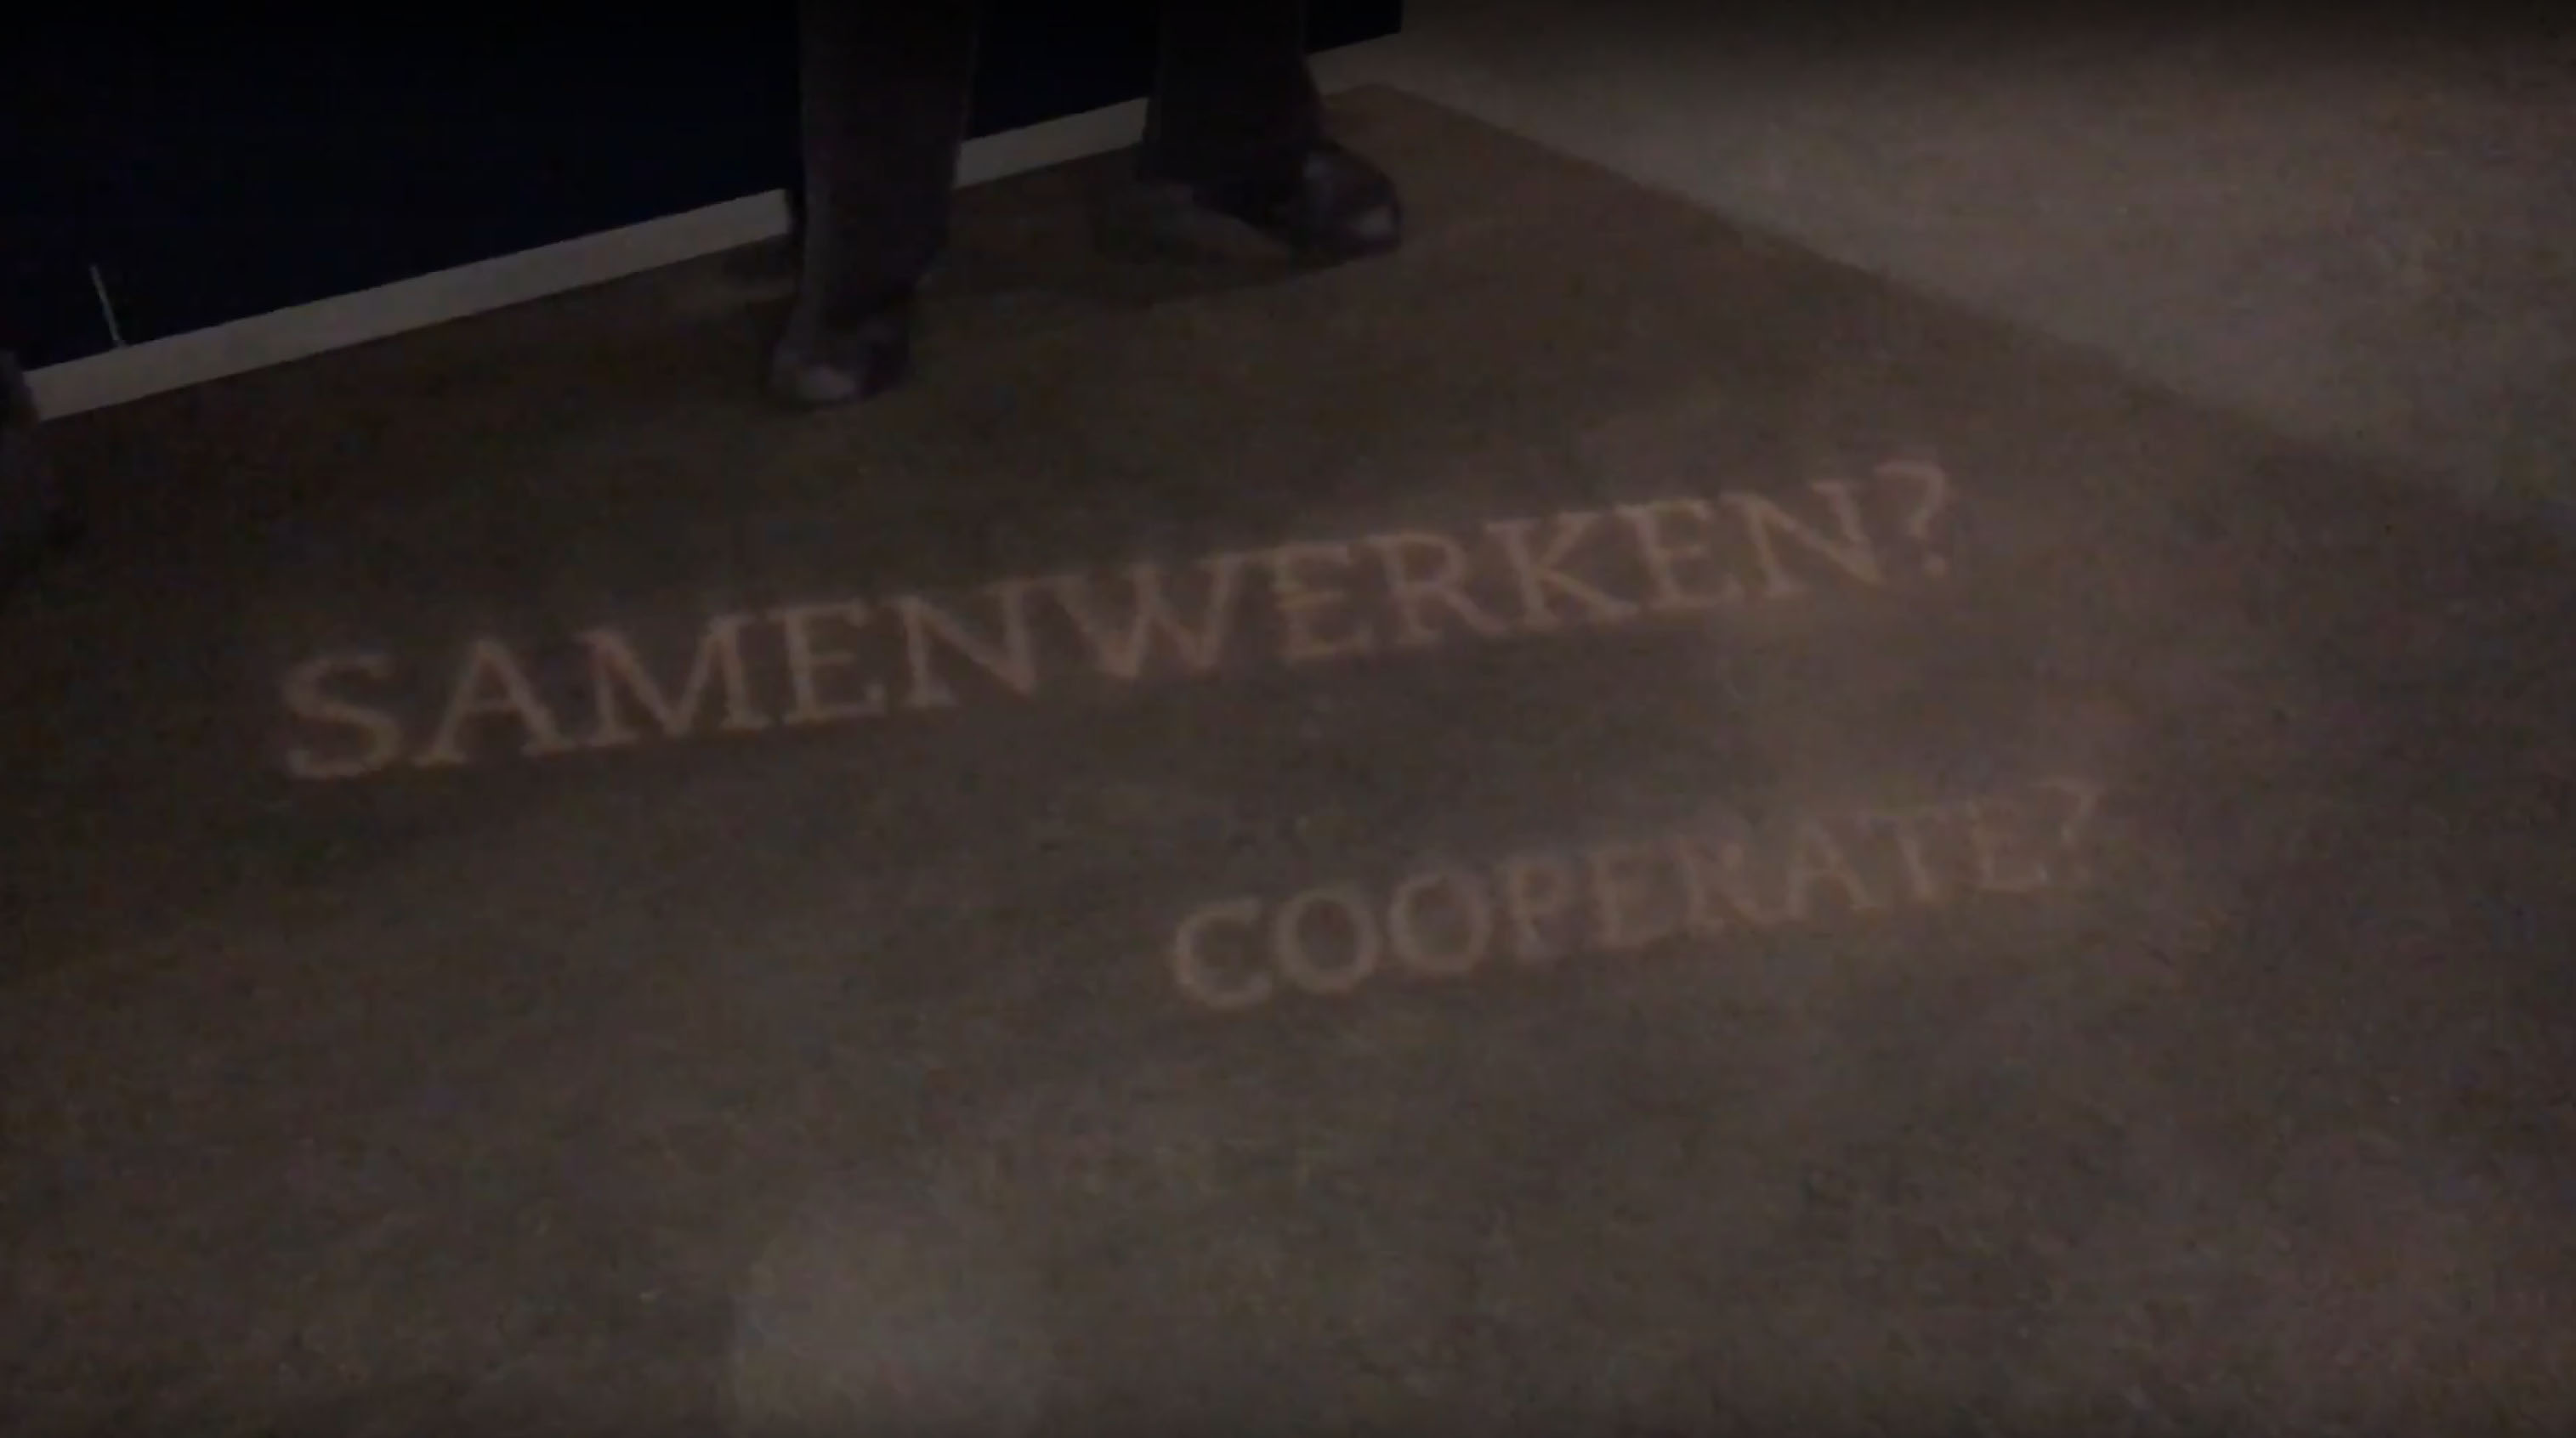
\includegraphics[width=8cm]{assets/dilemma.jpg}
\caption{The Current Representation of Dilemmas in the Dutch Resistance Museum}
\centering
\label{dilemma}
\end{figure}

\subsection{Methodological Approach} \label{Methodological Approach}
The exhibit is designed via a user-centered approach that constantly stays true to the user needs. User needs are assessed through participant observations and three rounds of user testing. User testing is carried out through experience testing with a qualitative and inductive approach and with constructivist and interpretivist perspectives.

The design process is carried out with help of the \textit{double diamond design process model} (Figure \ref{Diamond}). This model divides the design process into four stages: discover, define, develop and deliver. The stages of discover and define make up the conception phase, while the stages of develop and deliver make up the prototyping phase. Designed by the Design Council in 2005, the double diamond illustrates the creative process of going from various ideas (divergent thinking) to the best idea through refinement (convergent thinking)\cite{UKDesignCouncil2005AProcess}. 

\begin{figure} [H]
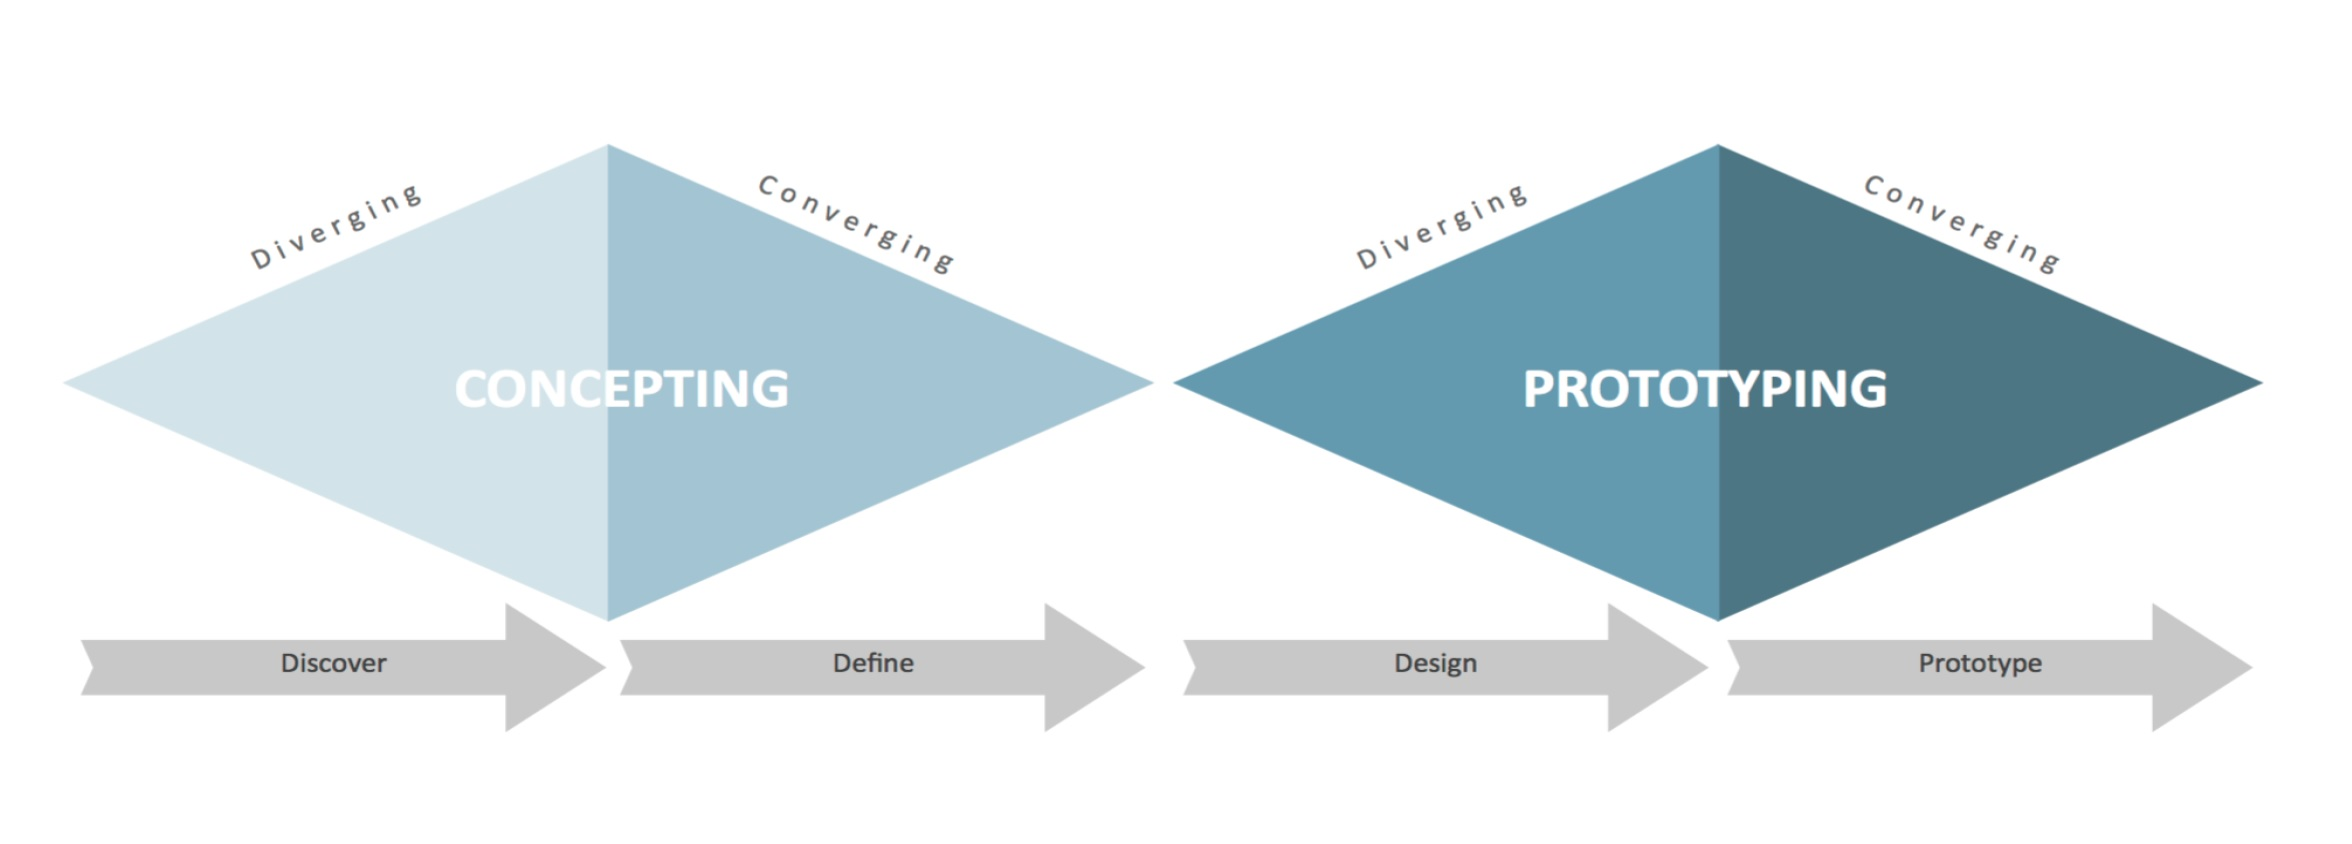
\includegraphics[width=8cm]{assets/diamond.jpg}
\caption{The Double Diamond Design Process Model (Informaat, 2017)}
\centering
\label{Diamond}
\end{figure}

\newpage
\section{Designing an Interactive Experience} \label{intexper}

Designing interactive components for the Dutch Resistance Museum exhibition was a collaborative process that was led by MSc students from the UvA \textit{Information Studies} master's programme and took place over five months. This section provides an overview of the process from concept (Section \ref{concept}) to a final interaction journey proposal (Section \ref{final_int_jour}) through the use of user needs and scenario (Section \ref{persona}), system requirements (Section \ref{sys_req}) and usability testing (Section \ref{US_TEST}).


\subsection{Concept} \label{concept}
Using the approach mentioned above (Section \ref{Methodological Approach}) a concept was created as a solution to the problem discussed in section \ref{Problem}. \textit{Identification Rumble} is a system that gives visitors of the Dutch Resistance Museum the opportunity to make choices people encountered during the occupation. The visitors get a replica of an identity card from that period. They use this item to register the choices they make while going through the exhibition. Dilemma stations are placed on multiple locations in the permanent exhibition. The dilemma station is an screen integrated in the interior of the exhibit. When visitors scan their identity card they are provided with an animation showing the visitor or group the context of the dilemma and a question. The visitor or group answer the question by scanning their identity card at the correspondent reader. They can visit as many dilemmas as they like. At the end of the exhibition the \textit{Evaluation Station} allows visitors to reflect on their choice, see potential consequences of their answers and compare their own decision to choices made by previous visitors.

\subsection{User Needs and Scenario} \label{persona}

\subsubsection{User Group}

The Dutch Resistance Museum attracts different kind of groups. One of the biggest groups of visitors is the English speaking tourist. As can be seen in (Figure \ref{Graphs}) 53\% of the visitors in 2016 originated from English speaking countries. This is followed by 26\% of visitors coming from the Netherlands and 20\% of visitors coming from other countries. The attraction the museum has on English speaking visitors is also visible in the language selection of audio guides. In 2016 a total of 50,160 audio guides were given to visitors. Of these audio guides 35,044 were in English, 4,812 in Dutch, 3,318 in German and the rest of the audio guides were set to other languages\cite{CommissariaatvoordeMedia2016}. The tourists that visit the museum are not particularly interested in internationally themed exhibitions. They almost exclusively visit the museum for the permanent exhibition which tells the Dutch story of the occupation during WWII\cite{VerzetsmuseumAmsterdam2017Ondernemingsplan2017-2020}. \\

Families with young children and school groups also visit the museum. Families with young children can go to the exhibition Dutch Resistance Museum Junior\footnote{\url{https://www.verzetsmuseum.org/museum/nl/verzetsmuseum-junior}, Accessed 09-02-2018} and the museum provides schools with special education programs. The system discussed in this paper focuses on the permanent exhibition of the museum. Therefore, families with young children and school groups are not the intended target user group of the system.

\begin{figure} [H]
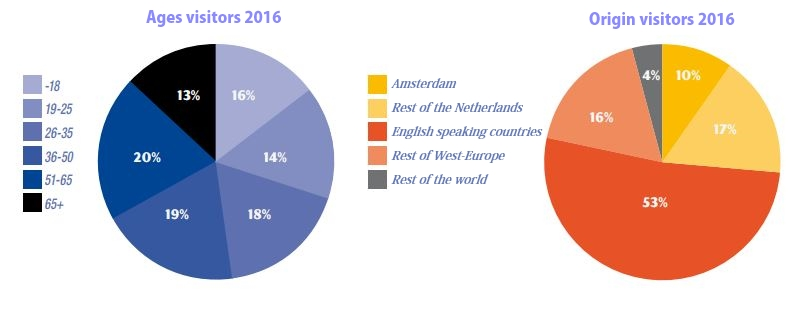
\includegraphics[width=7cm]{assets/Graphs.JPG}
\caption{Age and origin of Dutch Resistance Museum visitors\cite{CommissariaatvoordeMedia2016}}
\centering
\label{Graphs}
\end{figure}

\subsubsection{Persona} 
This section introduces a persona, named Tony the Tourist, to increase the understanding of the user group and their needs. Tony represents a range of museum visitors that will be interacting with Identification Rumble.\\

Tony is 36 years old and lives in Birmingham in the United Kingdom. He has a middle-range income and considers himself an environmentalist. He likes to read books, watch documentaries and travel. When he is traveling he likes to visit places featuring cultural heritage, for example museums. Tony is politically involved and is frustrated by environmental pollution and developments such as Brexit and the rising house prices.

\subsubsection{Scenario}

Tony and his girlfriend Emma go on a vacation to the Netherlands. They decide to visit the Dutch Resistance Museum in Amsterdam. Tony's grandparents survived WWII and he is interested in different points of views. When Tony and Emma enter the museum they buy a ticket at the front desk. The museum volunteer working at the desk asks the couple if they would like to go through the exhibition with \textit{Identification Rumble}, an interactive choice based experience. When Tony agrees the volunteer hands him a replica of an identity card that was used during WWII and explains that it functions as a tool for Tony to interact with the exhibition. The volunteer explains that they only get one identity card for both of them and that they will be using it to register choices they make as a group. The identity card is attached to a cord which Tony hangs around his neck. Before entering the exhibition, Tony comes across a language selection station prompting him to scan his identity card at his preferred language. Tony pushes his card against the reader underneath the symbol of the United Kingdom flag. Tony has been in Amsterdam for a few days and has had some experience with the public transport. He recognizes the movement of scanning the identity card being similar to using the public transport card. The language station emits a beeping noise confirming Tony's language selection.\\

Tony and Emma enter the exhibition and walk around. They come across a screen that is integrated into the interior of the exhibition. The screen prompts Tony to scan his identity card. He complies which in turn plays an animation on the screen. The animation starts off with a short text telling Tony and Emma that in the beginning of the occupation during WWII all civil servants were required to fill in ancestry forms. The animation proceeds to show people in a library having a conversation. They discuss whether the main character of the video, named Theo Inden, should fill in the form or not. Theo is Jewish and is worried about filling in the form. The other character in the animation is Theo's coworker, Johan, trying to persuade him to fill in the form. They debate their points of view and after that the library and Johan fade out. This leaves a prompt behind asking Tony and Emma what they would do in Theo's situation. They are encouraged to discuss if possible and to scan the identity card to register their choice. The options \textit{'Register'} and \textit{'Refuse'} are displayed on the screen being aligned with their corresponding card reader. Tony and Emma discuss the two options, the points that the characters in the video made and other arguments Tony and Emma came up with themselves. After a few minutes they decide to go for the \textit{'Refuse'} option. Tony scans the identity card by holding it against the reader aligned with the word \textit{'Refuse'} on the screen. The reader beeps to indicate that their choice has been registered. Before moving, along Emma points out to Tony the ancestry form that is being displayed near the screen. \\

Tony and Emma move through the exhibition while encountering other screens. More dilemmas are being presented to them in the same way as the \textit{'Register?'} dilemma. Each dilemma containing an animation with dialogue and a choice to be made. At some point in the exhibition, Tony comes across real identity cards that look very similar to the identity card he is carrying. Tony and Emma spend some time looking at the identity cards and reading about them.\\

At the end of the exhibit, Tony and Emma find another screen which is labeled \textit{Evaluation Station}. Tony scans the identity card once again. Some of the dilemmas Tony and Emma visited pop up on the screen. The dilemmas are shown next to each other horizontally and arrows on the both sides of the screen indicate that it would be possible to scroll through all the visited dilemmas. Tony touches the screen to do so. When he touches the dilemma \textit{'Register?'} the screen informs him which choice they made and how many visitors made the same choice. It also states that almost all civil servants in 1941 filled in the ancestry form which led to Jewish civil servants being fired the next month. Tony touches an arrow in the left top of the screen to return to the overview of the dilemmas. In the left bottom corner of the screen underneath the dilemmas Tony and Emma notice a column named consequences. This section informs them that the choices they made during the exhibit where rebellious but also increases the risk of not surviving WWII. They browse the dilemmas a couple minutes longer and then touch an arrow in the bottom right of the screen which reads \textit{'continue'}. They get the option to e-mail the results of their exhibit experience to themselves. They both fill in their e-mail addresses. Tony touches \textit{'continue'} once again. The screen thanks them for their visit and reminds them to return their identity card at the front desk. It promises Tony and Emma a discount on coffee in the restaurant next door if they return their identity card. Tony and Emma willingly do so and enjoy their coffee next door.

\newpage
% !TEX root = ./setup.tex

\subsection{System Requirements}
This project design poses a set of requirements for both the museum and its visitors.
For visitors, these requirements are mainly focused on the interactive procedure of going through the exhibition from beginning to end.
In order to realize the project, the museum has to meet administrative and technical prerequisites.
These requirements will be discussed from separate perspectives in the following sections.


\subsubsection{Visitor Requirements}
Visitors are able to pick up an identity card replica, containing an RFID tag, at the entry of the museum.
This is precisely where the museum already hands out audio tour devices.
It should be made clear that the identity card is the only item they need to interact with the exhibition during their visit.
Additional explanations are not necessary which is in line with the initial stakeholder's guidelines.
Naturally, visitors are expected to return their identity card at a designated collection point before leaving the museum.

When interacting with different stations of the exhibition visitors should understand the main interaction of holding their identity card to scanner points.
Holding an identity card within the proximity of an RFID reader is the central action carried through the exhibition.
It either triggers the start of a station or signifies confirmation of a choice made by the visitor.
In addition to that, visitors need to recognize interaction points or namely where identity cards will be recognized.
Understanding this interaction will be supported by visual aids near interaction points and audiovisual feedback from stations.


\subsubsection{Museum Requirements}
The museum has to build props (identity cards), acquire necessary hardware (stations), setup software system and produce digital material (dilemma animations) to realize the project.

Identity cards are set together by equipping a physical replica with an RFID tag.
Therefore, custom replicas have to be assembled mimicking the look and haptic of identity cards used during WWII.
Quality of these props can range from simple paper printouts to elaborate duplicates using leather covers.
This can be made dependant on the available budget.
On the technical side, RFID tags are easily acquired through local or online retail businesses.

Each station requires a specific hardware setup including RFID readers, screens and computers.
Language choice is backed by a single computer connected to an RFID reader per supported language of the museum.
Dilemma stations rely on a screen for playing their respective animation, a computer and an RFID reader per answer of the dilemma.
The evaluation station consists of a screen, computer and single RFID reader recognizing visitors with their identity card.

As the stations are at different locations within the museum one backend server acts as the communication hub.
This server needs to be setup one time by pulling the project's repository\footnote{\url{https://github.com/marc1404/identification-rumble}, Accessed: 09-02-2018} and installing Node.js\footnote{\url{https://nodejs.org/en/}, Accessed: 09-02-2018} as the runtime framework.
Needless to say, it should be kept running to render the exhibition stations usable and administrative interfaces available.
In order to connect the stations to the server, an internal network has to be provided.
It is not advisable to open the server to the public internet as this would open it up to malicious attacks.

Finally, each dilemma features an animated video with audio which guides visitors through the scenario.
These clips have to be produced from a technical side but also require voice actors to record narration and dialogue.
Furthermore, they should be available in all languages which the museum seeks to offer the exhibition in.
 \label{sys_req}


\subsection{Usability Testing} \label{US_TEST}
The project went through three rounds of usability testing. Each round produced feedback that in turn allowed to further refine the prototype. This section discusses each of these iteration rounds, their objectives, the feedback that was collected and their effects on the prototype.

\subsubsection{Iteration I}
The first iteration round started with the usability testing of a low-fidelity paper prototype. The main objective of this testing round was to reflect on the interactions and the ease of use of the design. The low-fidelity paper prototype included: one paper passport, one paper scanner, one A4 paper representing the starting screen and multiple A4 papers with a written out preliminary animation. Two test sessions were carried out during this testing round. Each session commenced with setting the scene. Once test participants understood their role as museum visitors they were asked to let the paper prototype guide them through the process.

\begin{figure} [h]
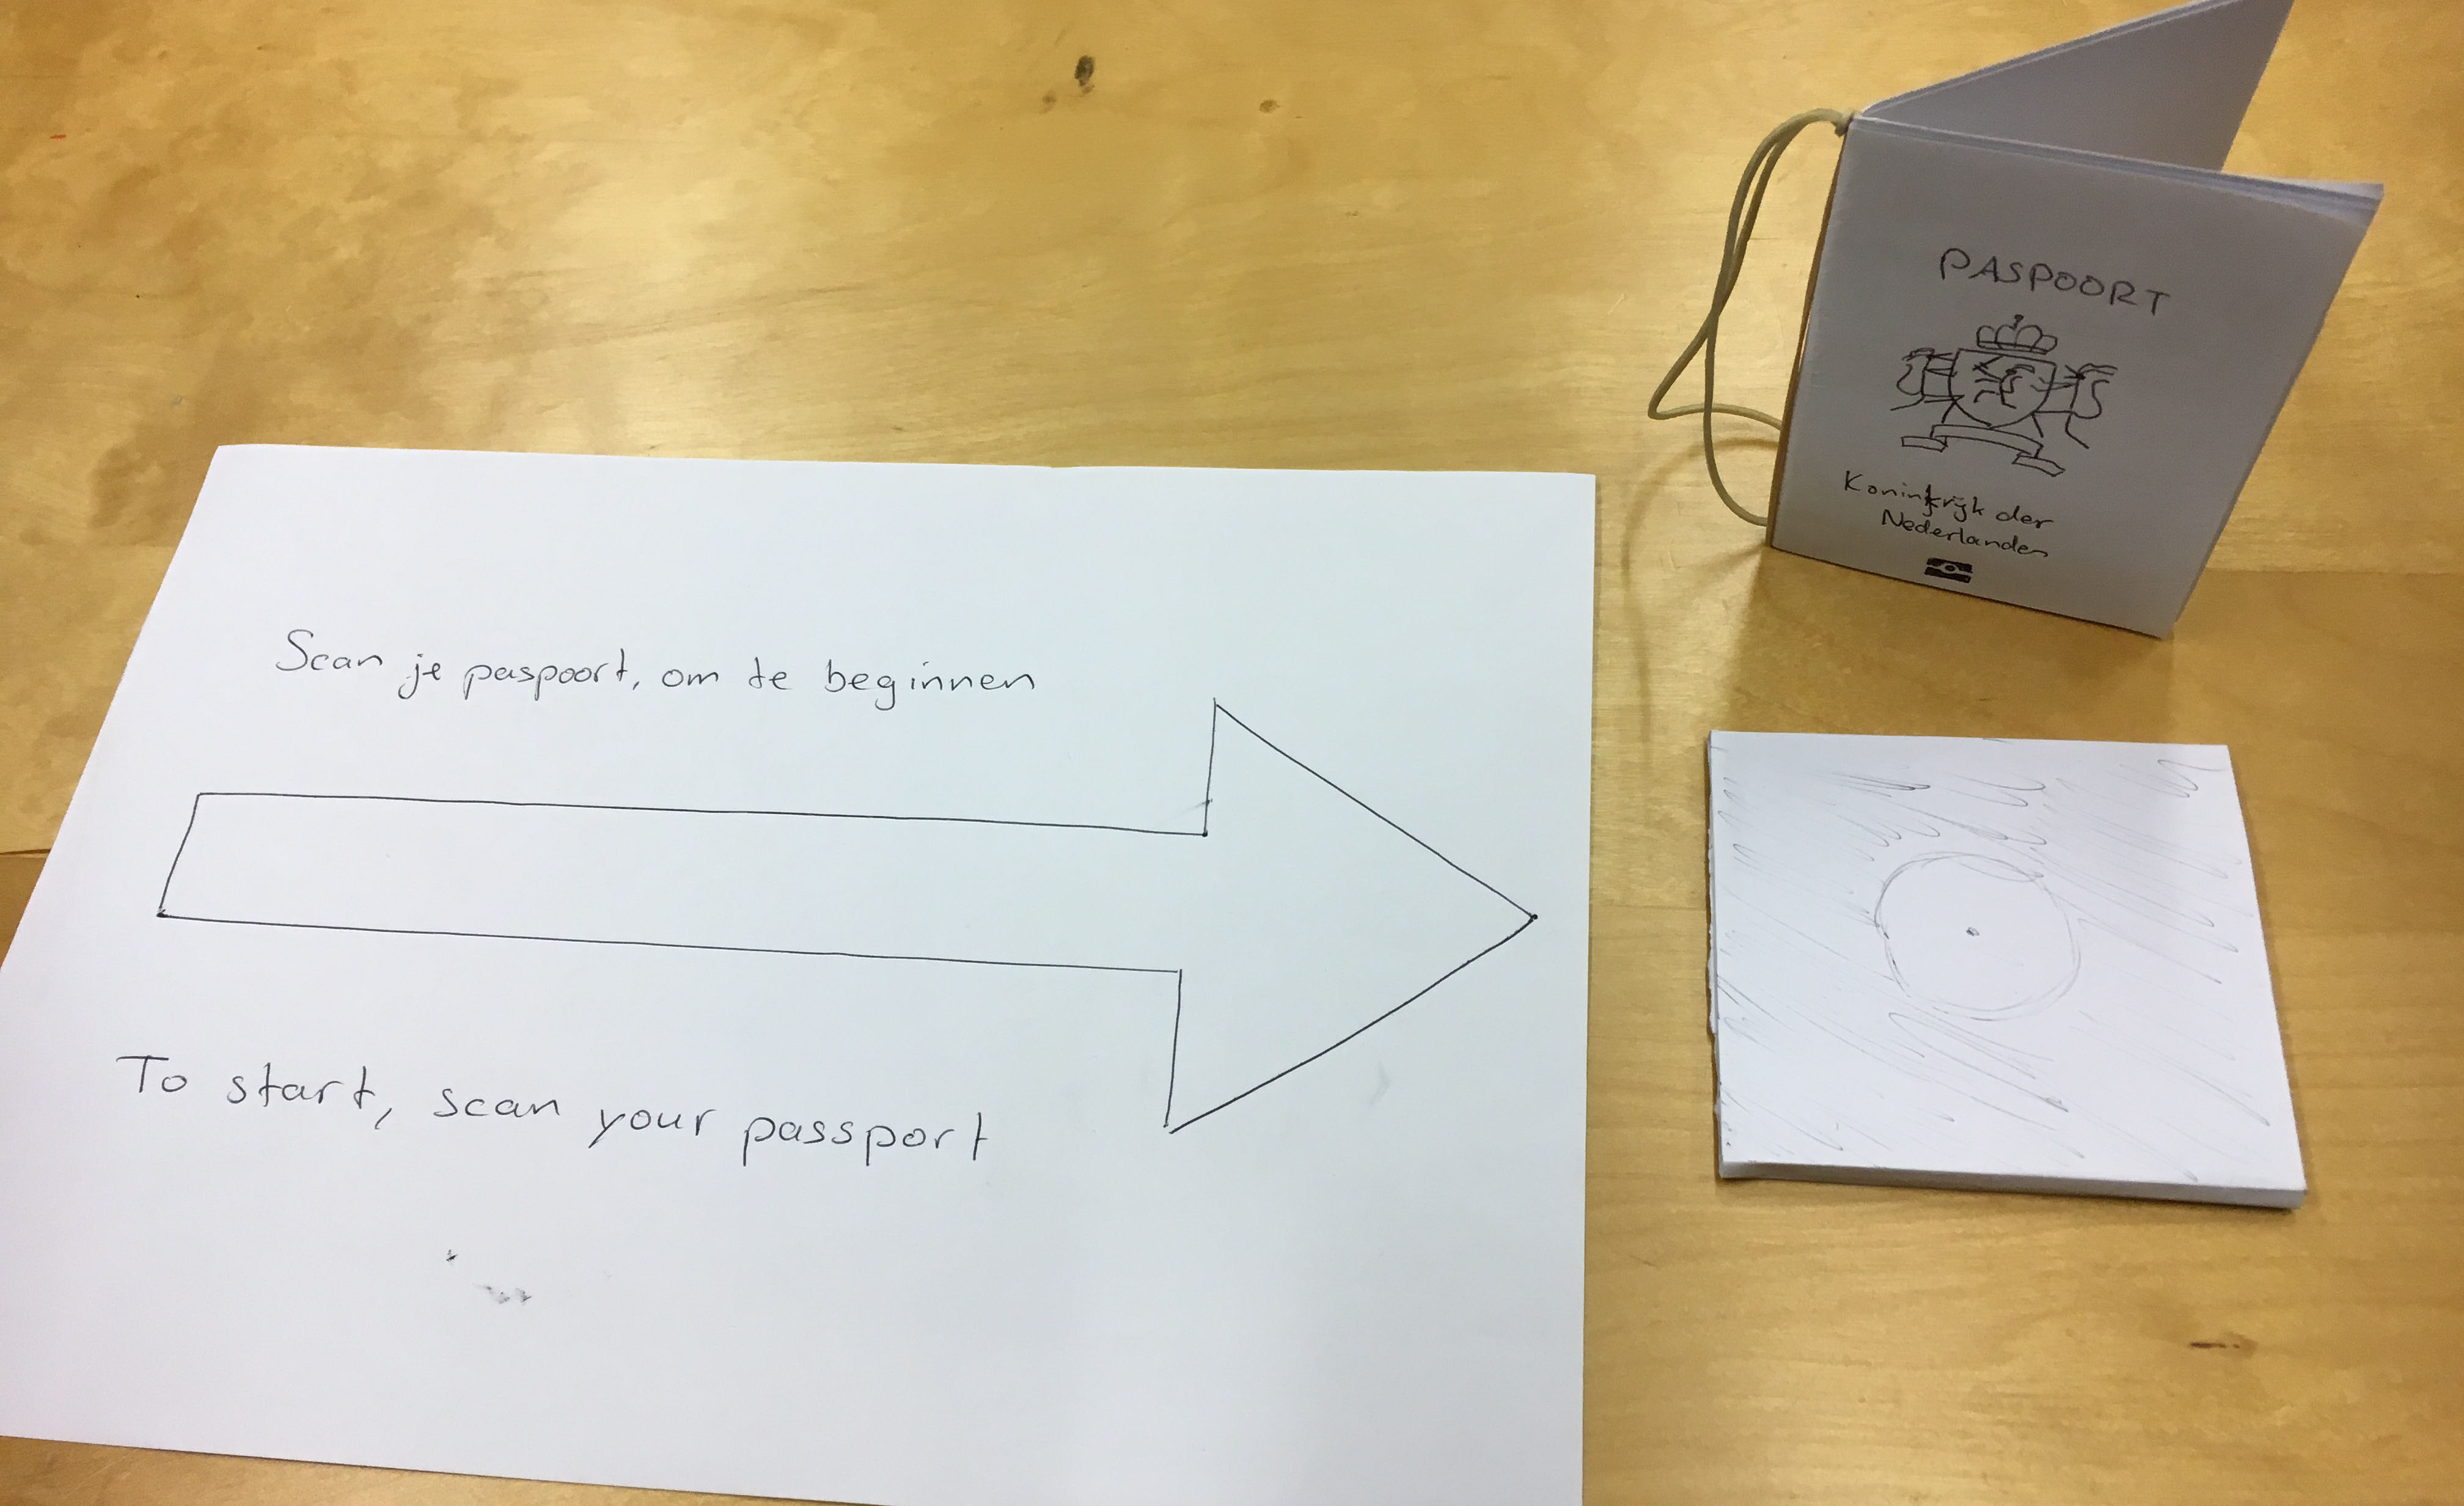
\includegraphics[width=8cm]{assets/paper_pro.JPG}
\caption{Low-Fidelity Paper Prototype}
\centering
\label{low_fi}
\end{figure}

Feedback showed that the intended interactions were clear and felt natural but that it was unclear how visitors or groups were supposed to make decisions with only one scanner on the wall and no buttons to make choices apparent. Due to the textual nature of the animation, test participants expressed their concern regarding the amount of text that was used to introduce the dilemma.

\subsubsection{Technical Prototype} The feedback from the low-fidelity prototype testing sessions was used to refine the design and served as input for the technical prototype. The choice to include not one but two dilemmas in the prototype was made to communicate the idea of an interactive experience more effectively. A QR-code on a mobile phone was introduced to simulate a situation where visitors can choose their own answer by scanning a passport. Passport scanning was replicated by scanning the QR-code with help of a web-cam (Figure \ref{QR_fi}). The QR-code was linked to a passport and kept track of language preference and dilemma choices. By linking a language preference to a passport, visitors are enabled to watch animations in their preferred language. The technical prototype was designed as a web-application.

\begin{figure} [h]
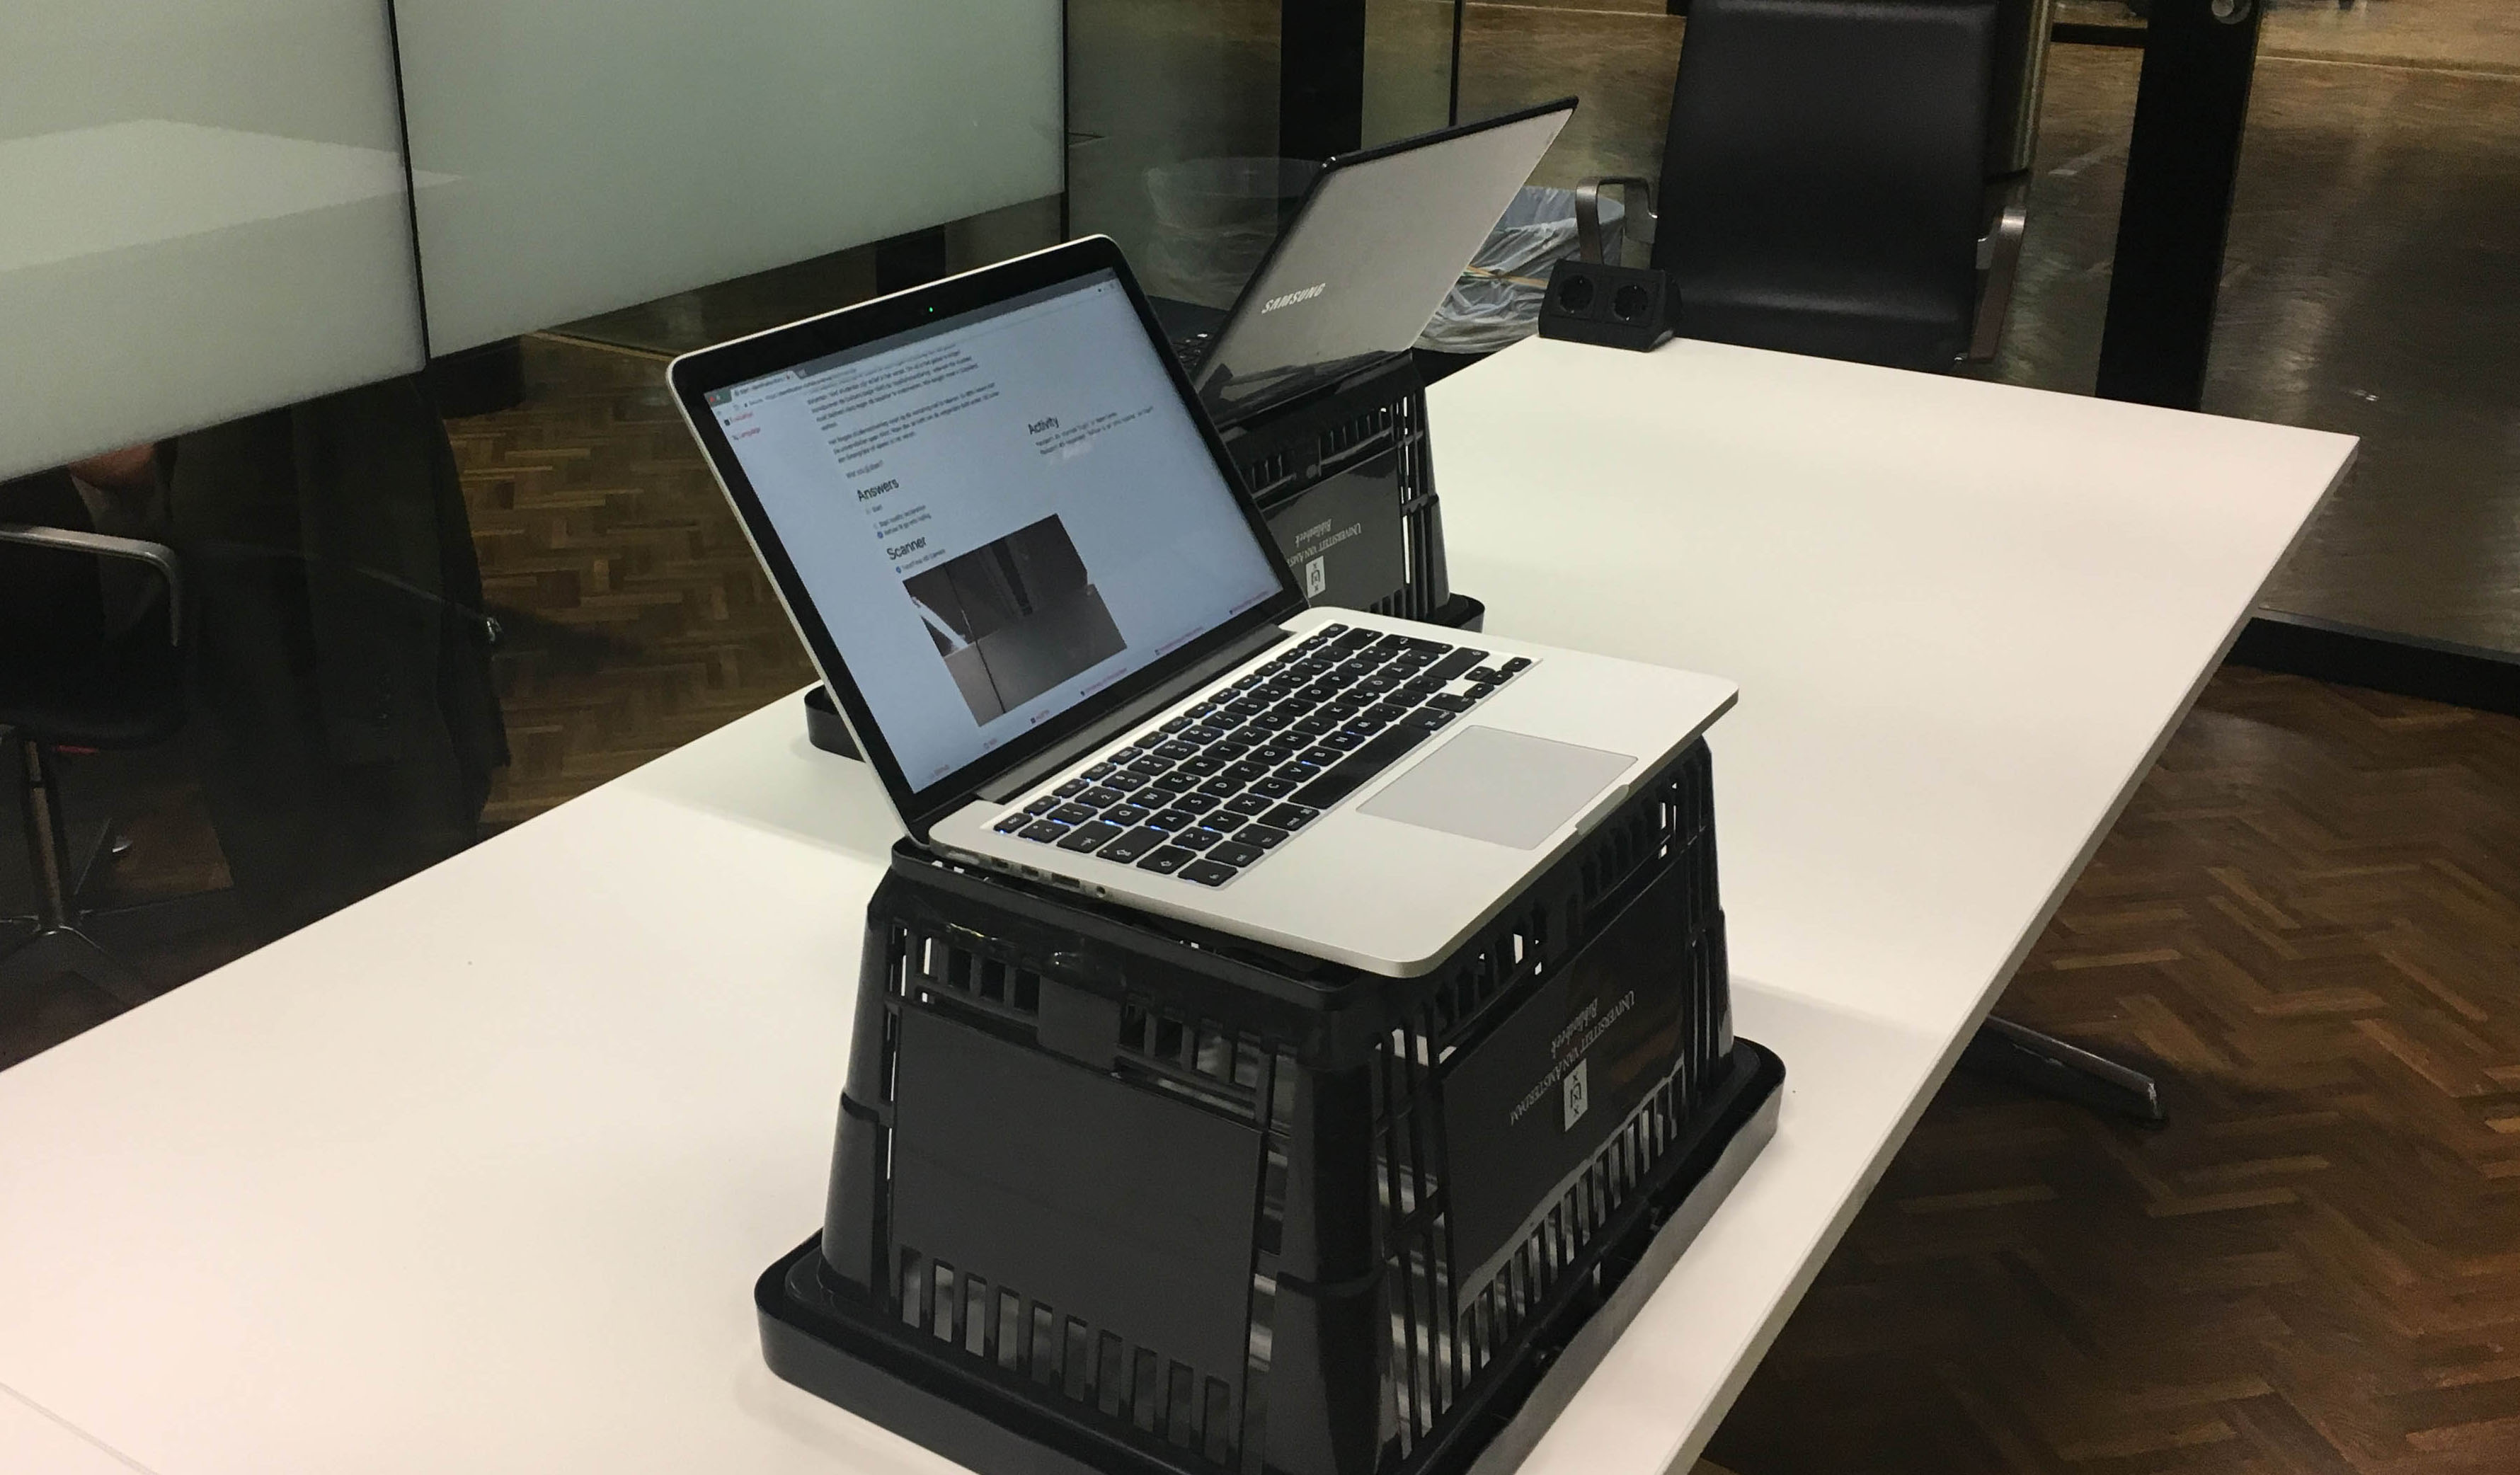
\includegraphics[width=8cm]{assets/first-ux-test.JPG}
\caption{Technological Prototype Testing Set-Up}
\centering
\label{tech_fi}
\end{figure}

\subsubsection{Iteration II}
The second iteration round started with the usability testing of the technical prototype. The main objective of this testing round was to reflect on the interactions, the idea of giving visitors a journey and the technology behind it all. To give test participants the impression that they were testing an interactive museum experience, the second usability testing round was executed with two laptops each representing a different dilemma station (Figure \ref{tech_fi}). Test participants were given four tasks: choose the language of the passport, go to the first dilemma station, go to the second dilemma station and proceed to the evaluation station.

Four test sessions were carried out during this test round. Each session commenced with a briefing that explained the museum context and the QR-code mechanism. Hereafter testing participants were asked to sign a consent form declaring that recordings and feedback may be used in an anonymized way. Test participants were asked to switch laptops after each action was completed, to think out loud and to take into account that this prototype was purely technical and far from the fully realized idea.

\begin{figure} [h]
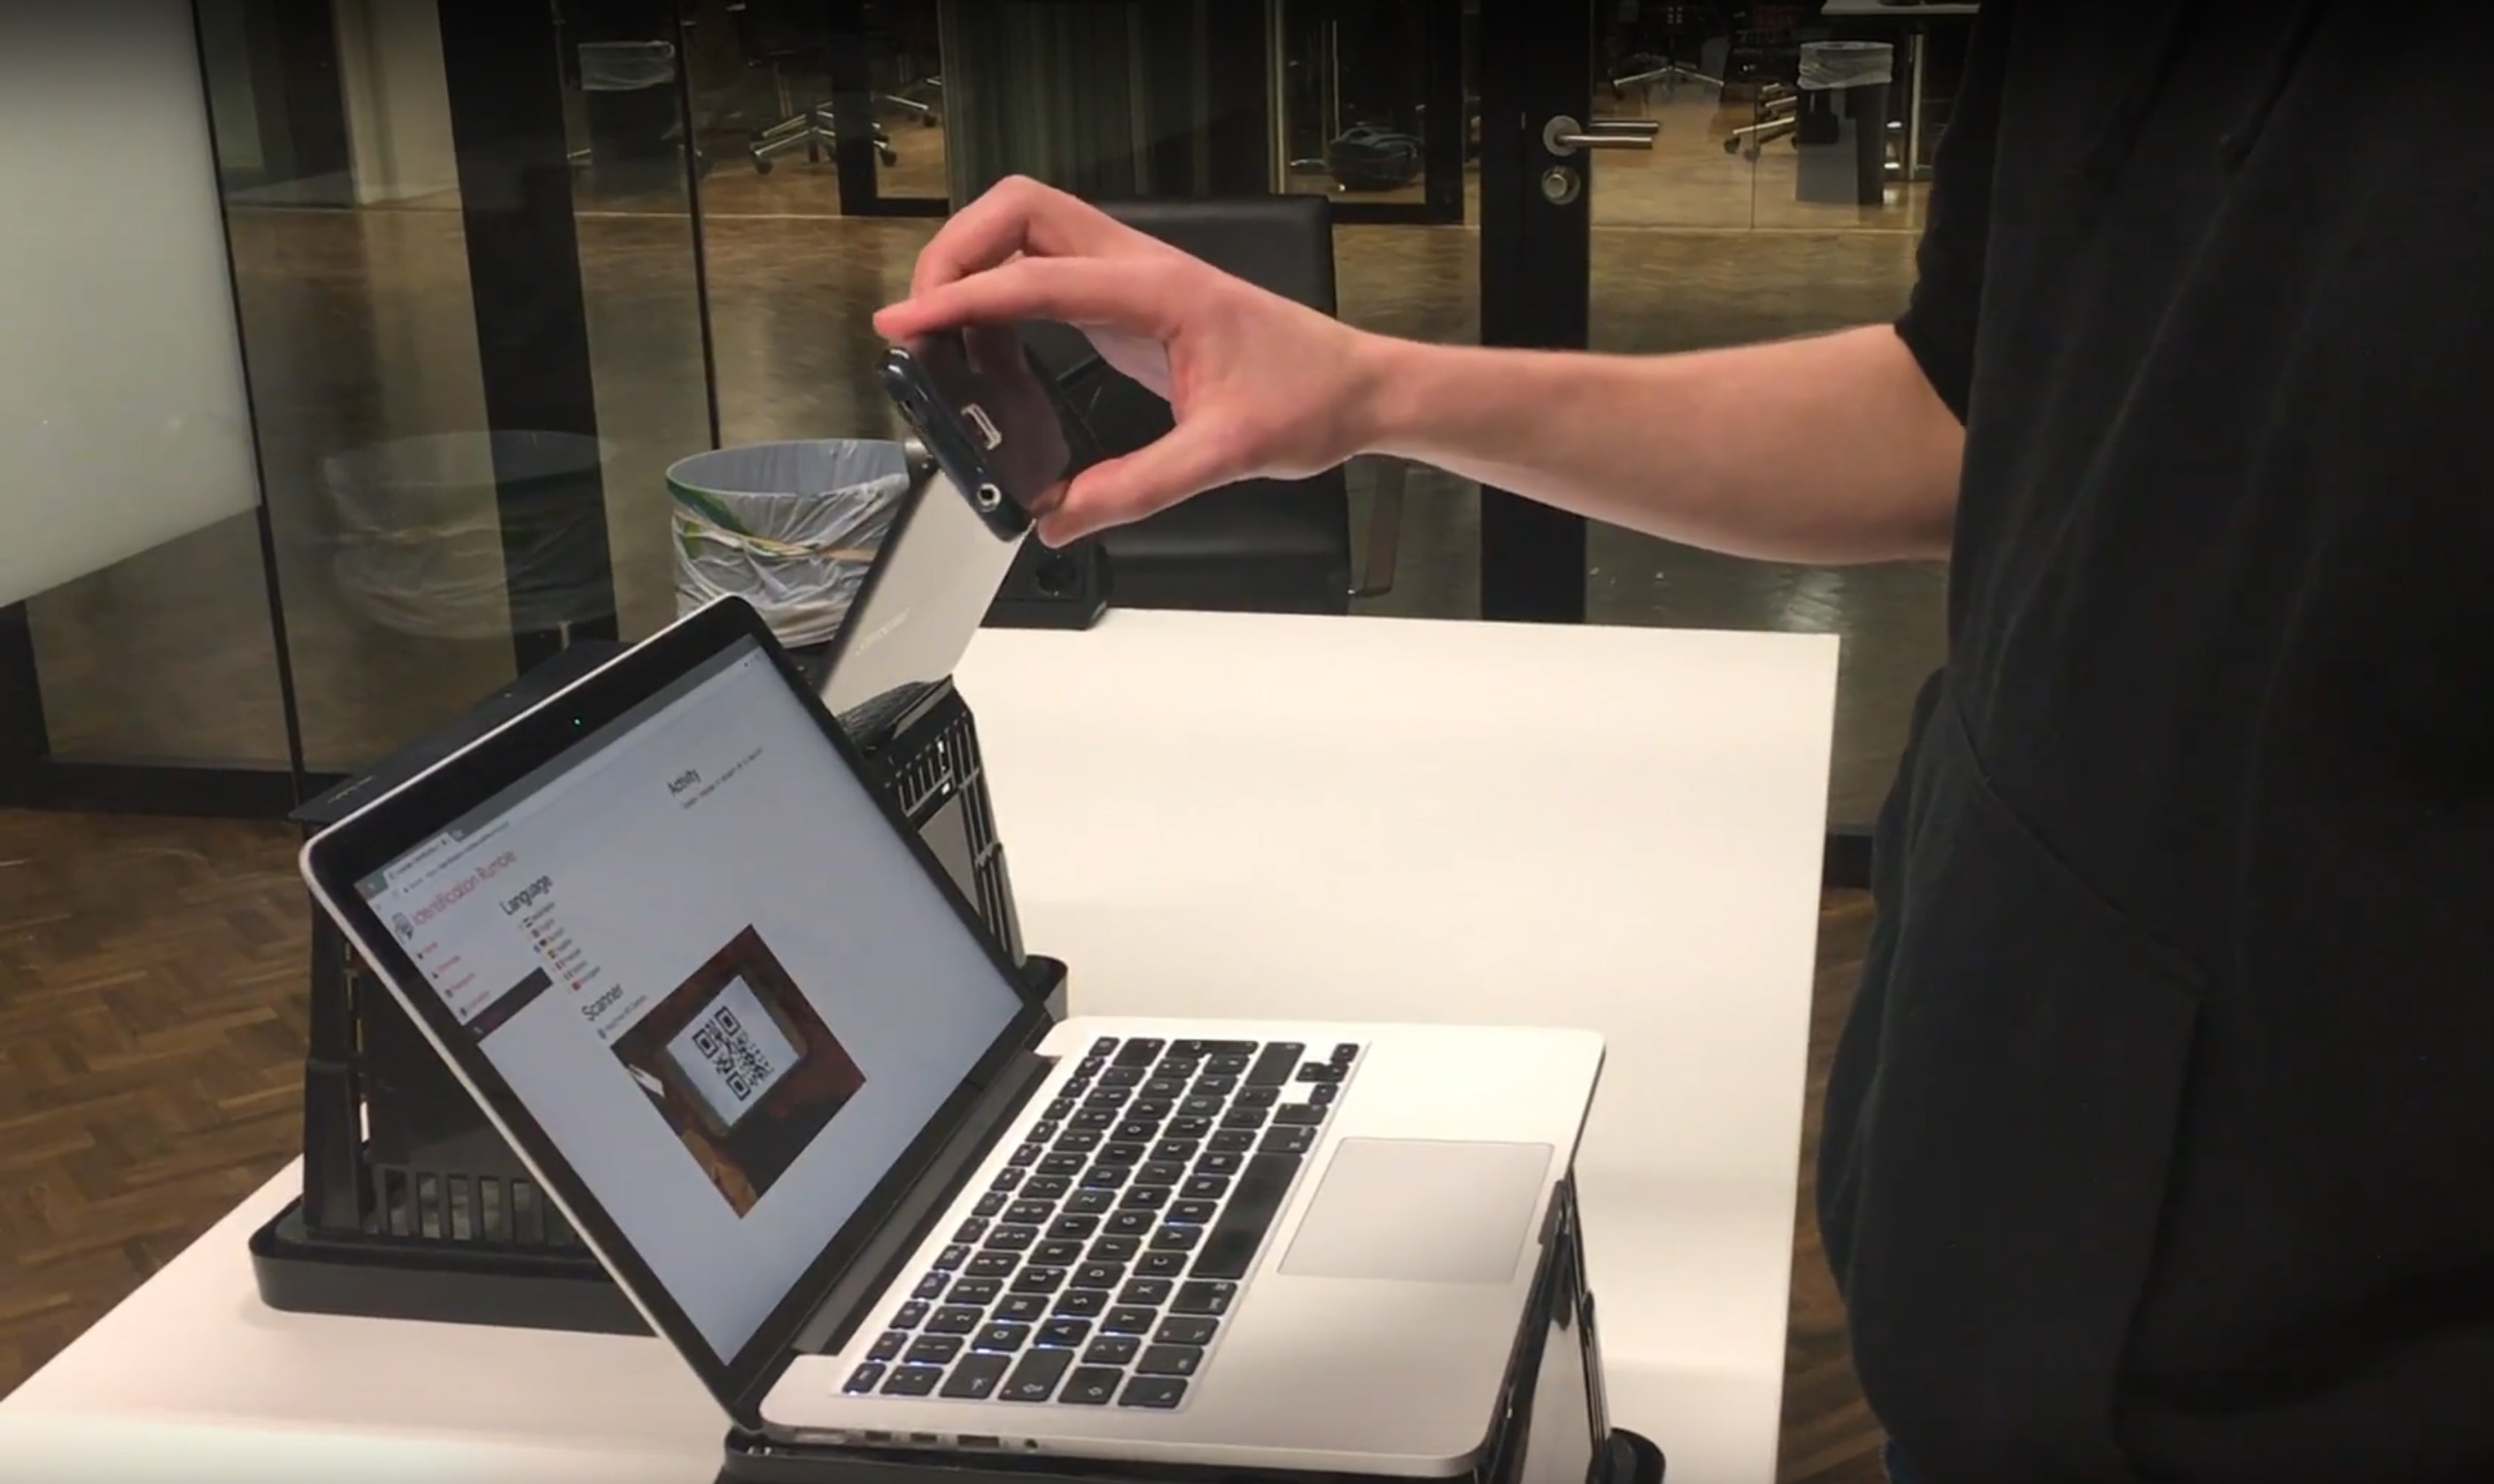
\includegraphics[width=8cm]{assets/test_QR2.jpg}
\caption{Technological Prototype Testing QR Scanning}
\centering
\label{QR_fi}
\end{figure}

Feedback from this test session emphasized that the binary choice (register or not) to conclude a dilemma station was perceived as pleasant and that walking around the room from station to station added to simulating walking around the exhibition. However, scanning the passport did not feel rewarding and a feedback beep was suggested. test participants also expressed feelings of incompleteness after answering a dilemma and suggested more feedback. The evaluation station at the end of the museum visit got a lot of positive feedback and test participants were very interested in seeing the choices that other visitors had made before them.

\subsubsection{Functional Prototype} The feedback collected during the second usability testing rounds was used to refine the design and served as input for the functional prototype. To give the prototype a more finalized look and feel, a carton box was decorated with wallpaper and cut in such a matter that it fit around a laptop screen. This way the laptop behaved and looked like a television screen as if already integrated into the exhibition (Figure \ref{Final_setup}). Only one RFID reader was available for this project, therefore two paper RFID readers simulated real life scanners. Instead of a textual dilemma introduction the main dilemma, \textit{'Register?'}, is now introduced through an animation wherein two characters have a conversation about the situation surrounding the dilemma\footnote{\url{https://identification-rumble.science/dilemmas/register}, Accessed 30-01-2018}. The second dilemma, \textit{'Sign?'}, was kept as part of the prototype in textual form because test participants remarked that it indeed gave them a better grasp of the interactive museum experience as opposed to only showing one dilemma. Moreover, to keep the passport replica historically correct, it became an identity card\footnote{\url{https://identification-rumble.science/persoonsbewijs}, accessed 06/02/2018} with an RFID chip embedded (Section \ref{System_Description}). Finally, the evaluation station was added to the end of the experience as proposed by multiple test participants to enable a moment of reflection, comparison and to give visitors an idea of how their choices could have influenced someone's life during that period.

\begin{figure} [h]
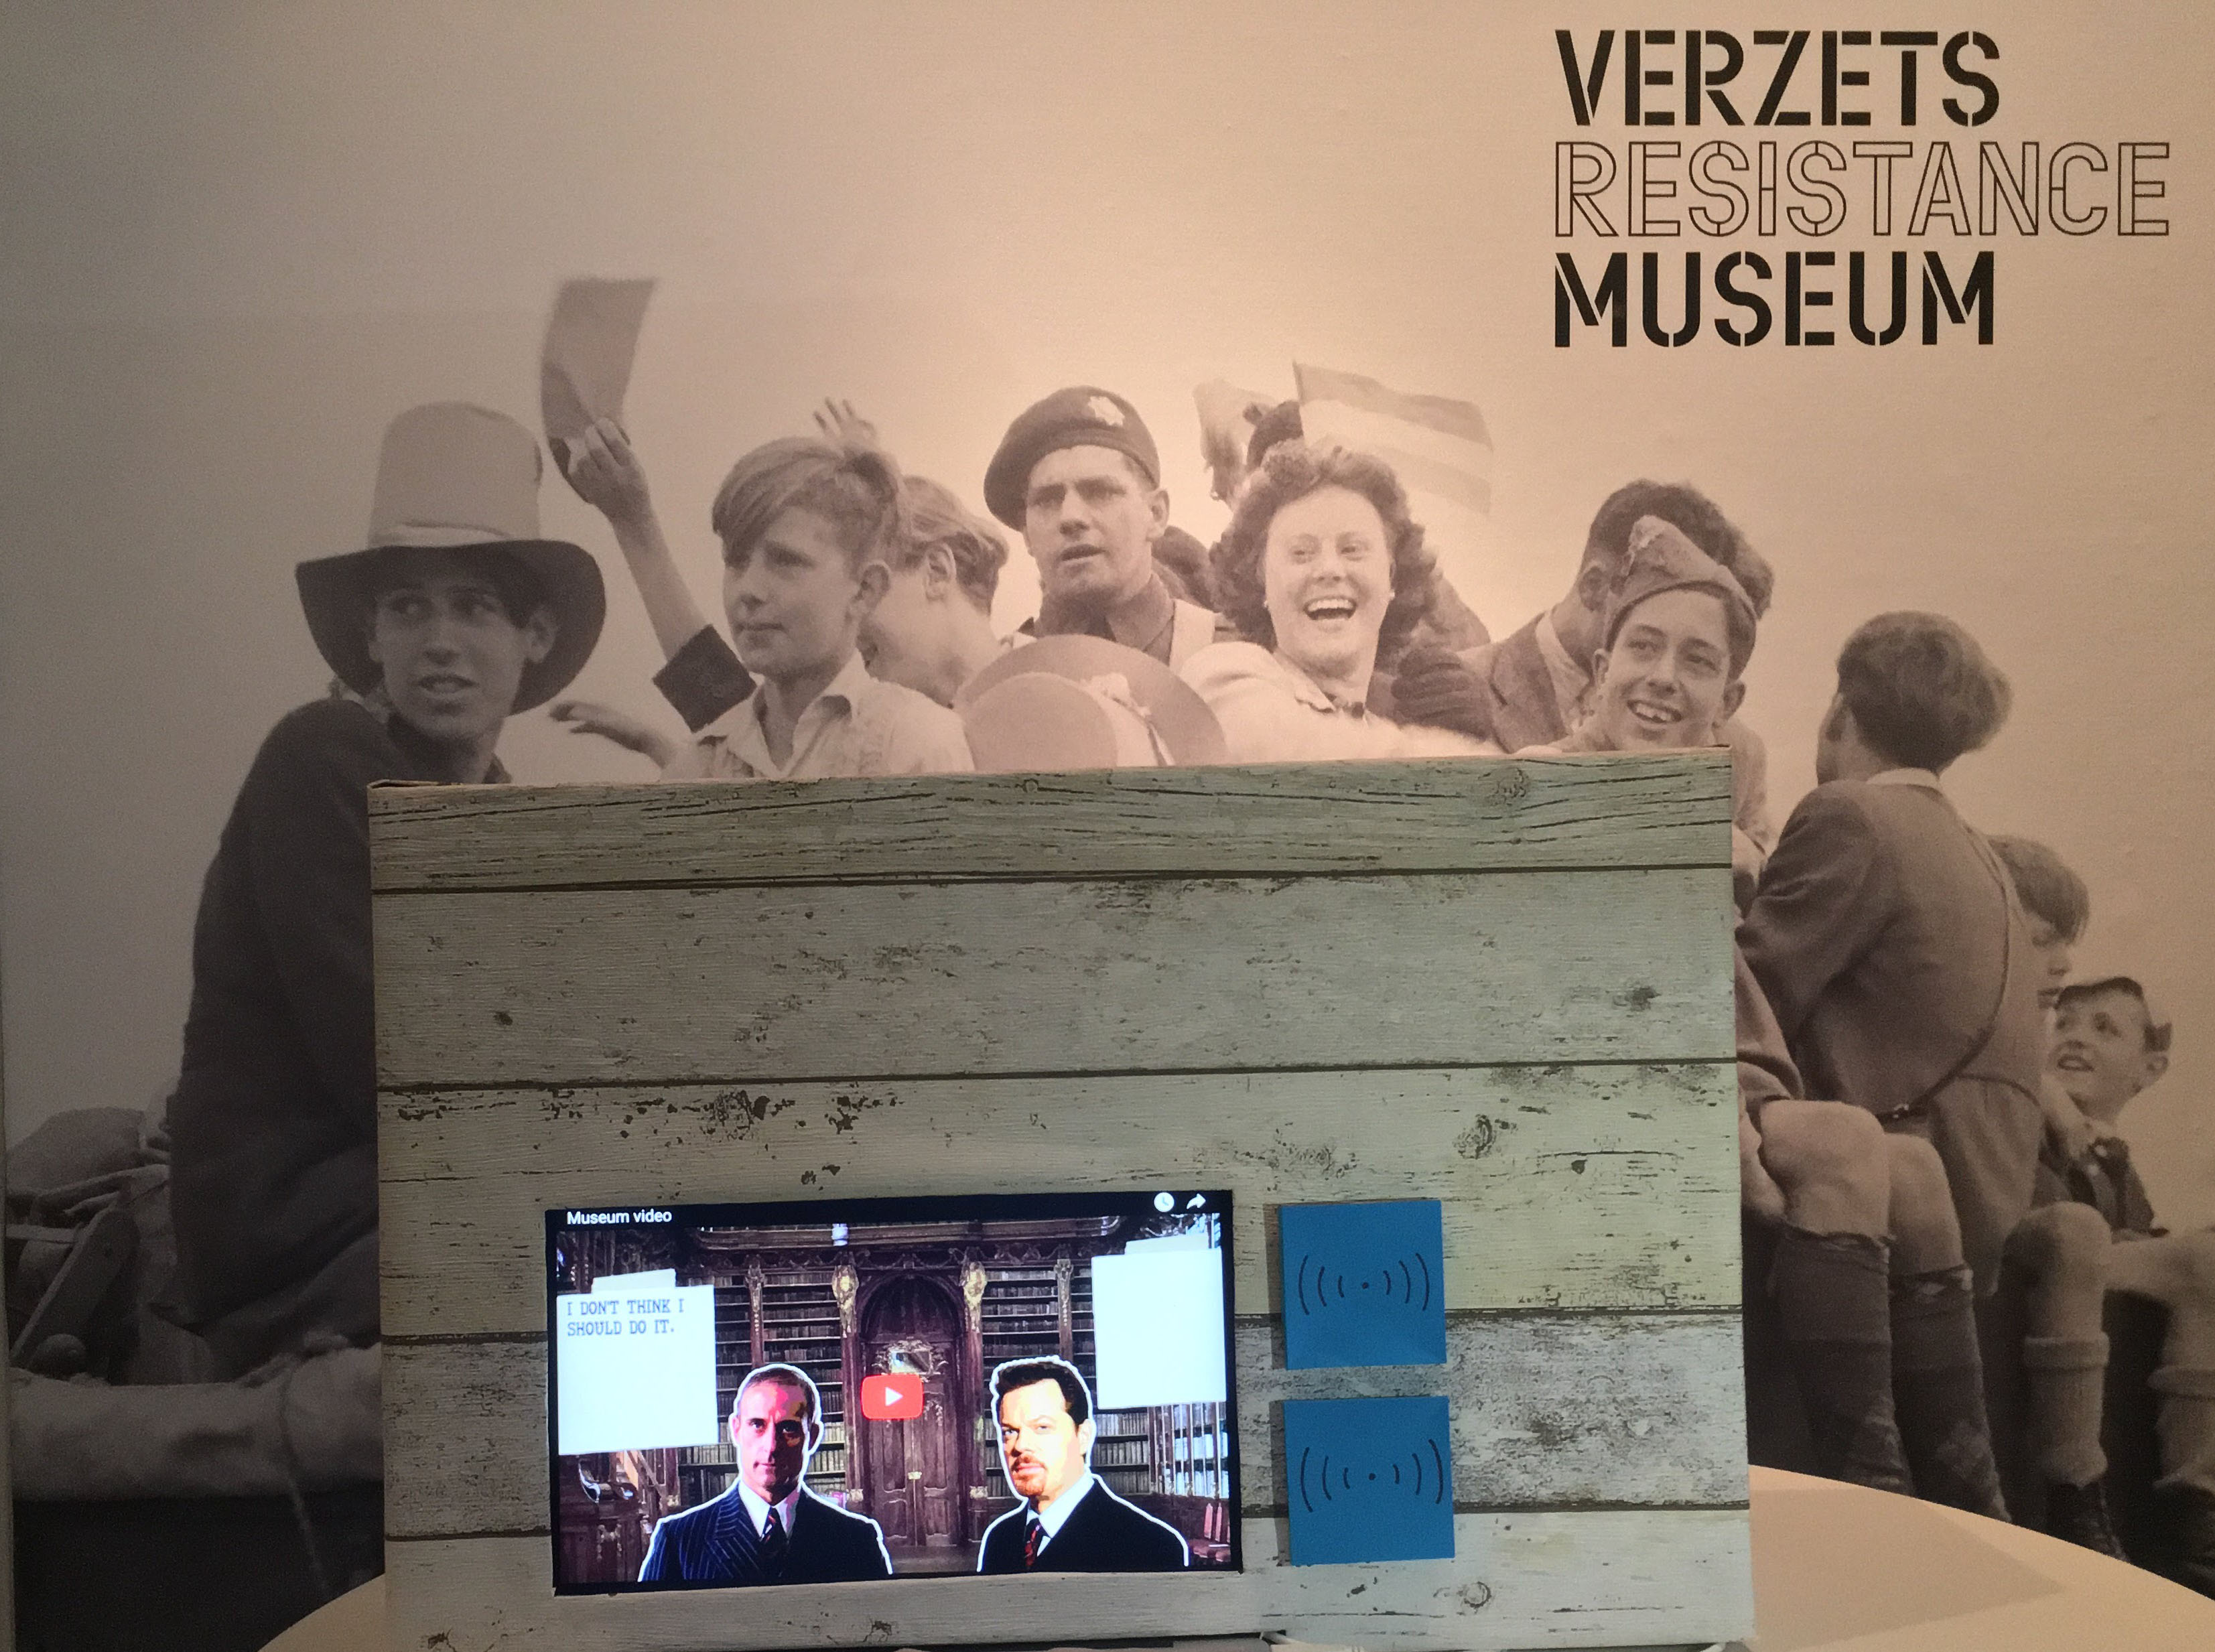
\includegraphics[width=8cm]{assets/prototype-in-museum-far.jpg}
\caption{Functional Prototype Test Setup}
\centering
\label{Final_setup}
\end{figure}

\subsubsection{Iteration III}
The third and last iteration round started with the usability testing of a functional prototype (Figure \ref{Final_setup}). The main objective of this testing round was to see if real visitors of the Dutch Resistance Museum understood the concept, objective and interactions of the Identification Rumble exhibit. The functional prototype entailed one cardboard box decorated with wallpaper and two dummy RFID scanners, one RFID scanner lined up behind the dummy scanners (Figure \ref{Box_Draw}), one laptop hooked up to a RFID scanner, two identity card replicas with embedded RFID chips. The prototype exhibit was set up in the main hall of the museum across the language activation wall (Figure \ref{INT_MAP}, point B). All testing participants signed a consent form declaring that recordings and feedback may be used in an anonymized way.

\begin{figure} [h]
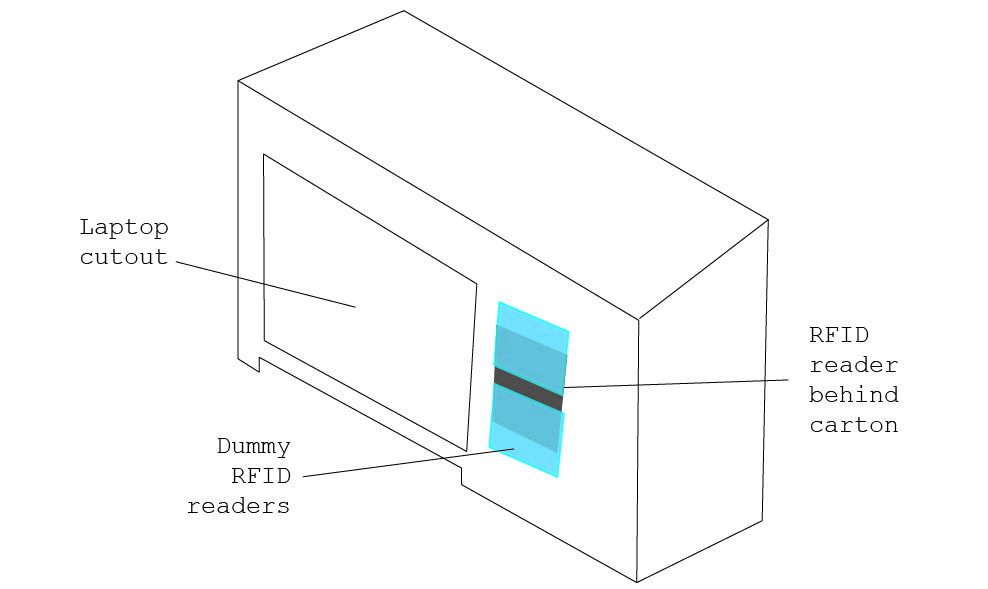
\includegraphics[width=8cm]{assets/box_draw.jpg}
\caption{Line Drawing of Functional Prototype with Placement of the Scanners}
\centering
\label{Box_Draw}
\end{figure}

Ten test sessions were carried out during this test round of which two involved a group of two people. Each session commenced with a briefing explaining the concept, context and further testing procedure. Hereafter, test participants were given four tasks: activate the identity card by choosing a preferred language, complete the first dilemma station, complete the second dilemma station and finally, proceed to the evaluation station.

\begin{figure} [h]
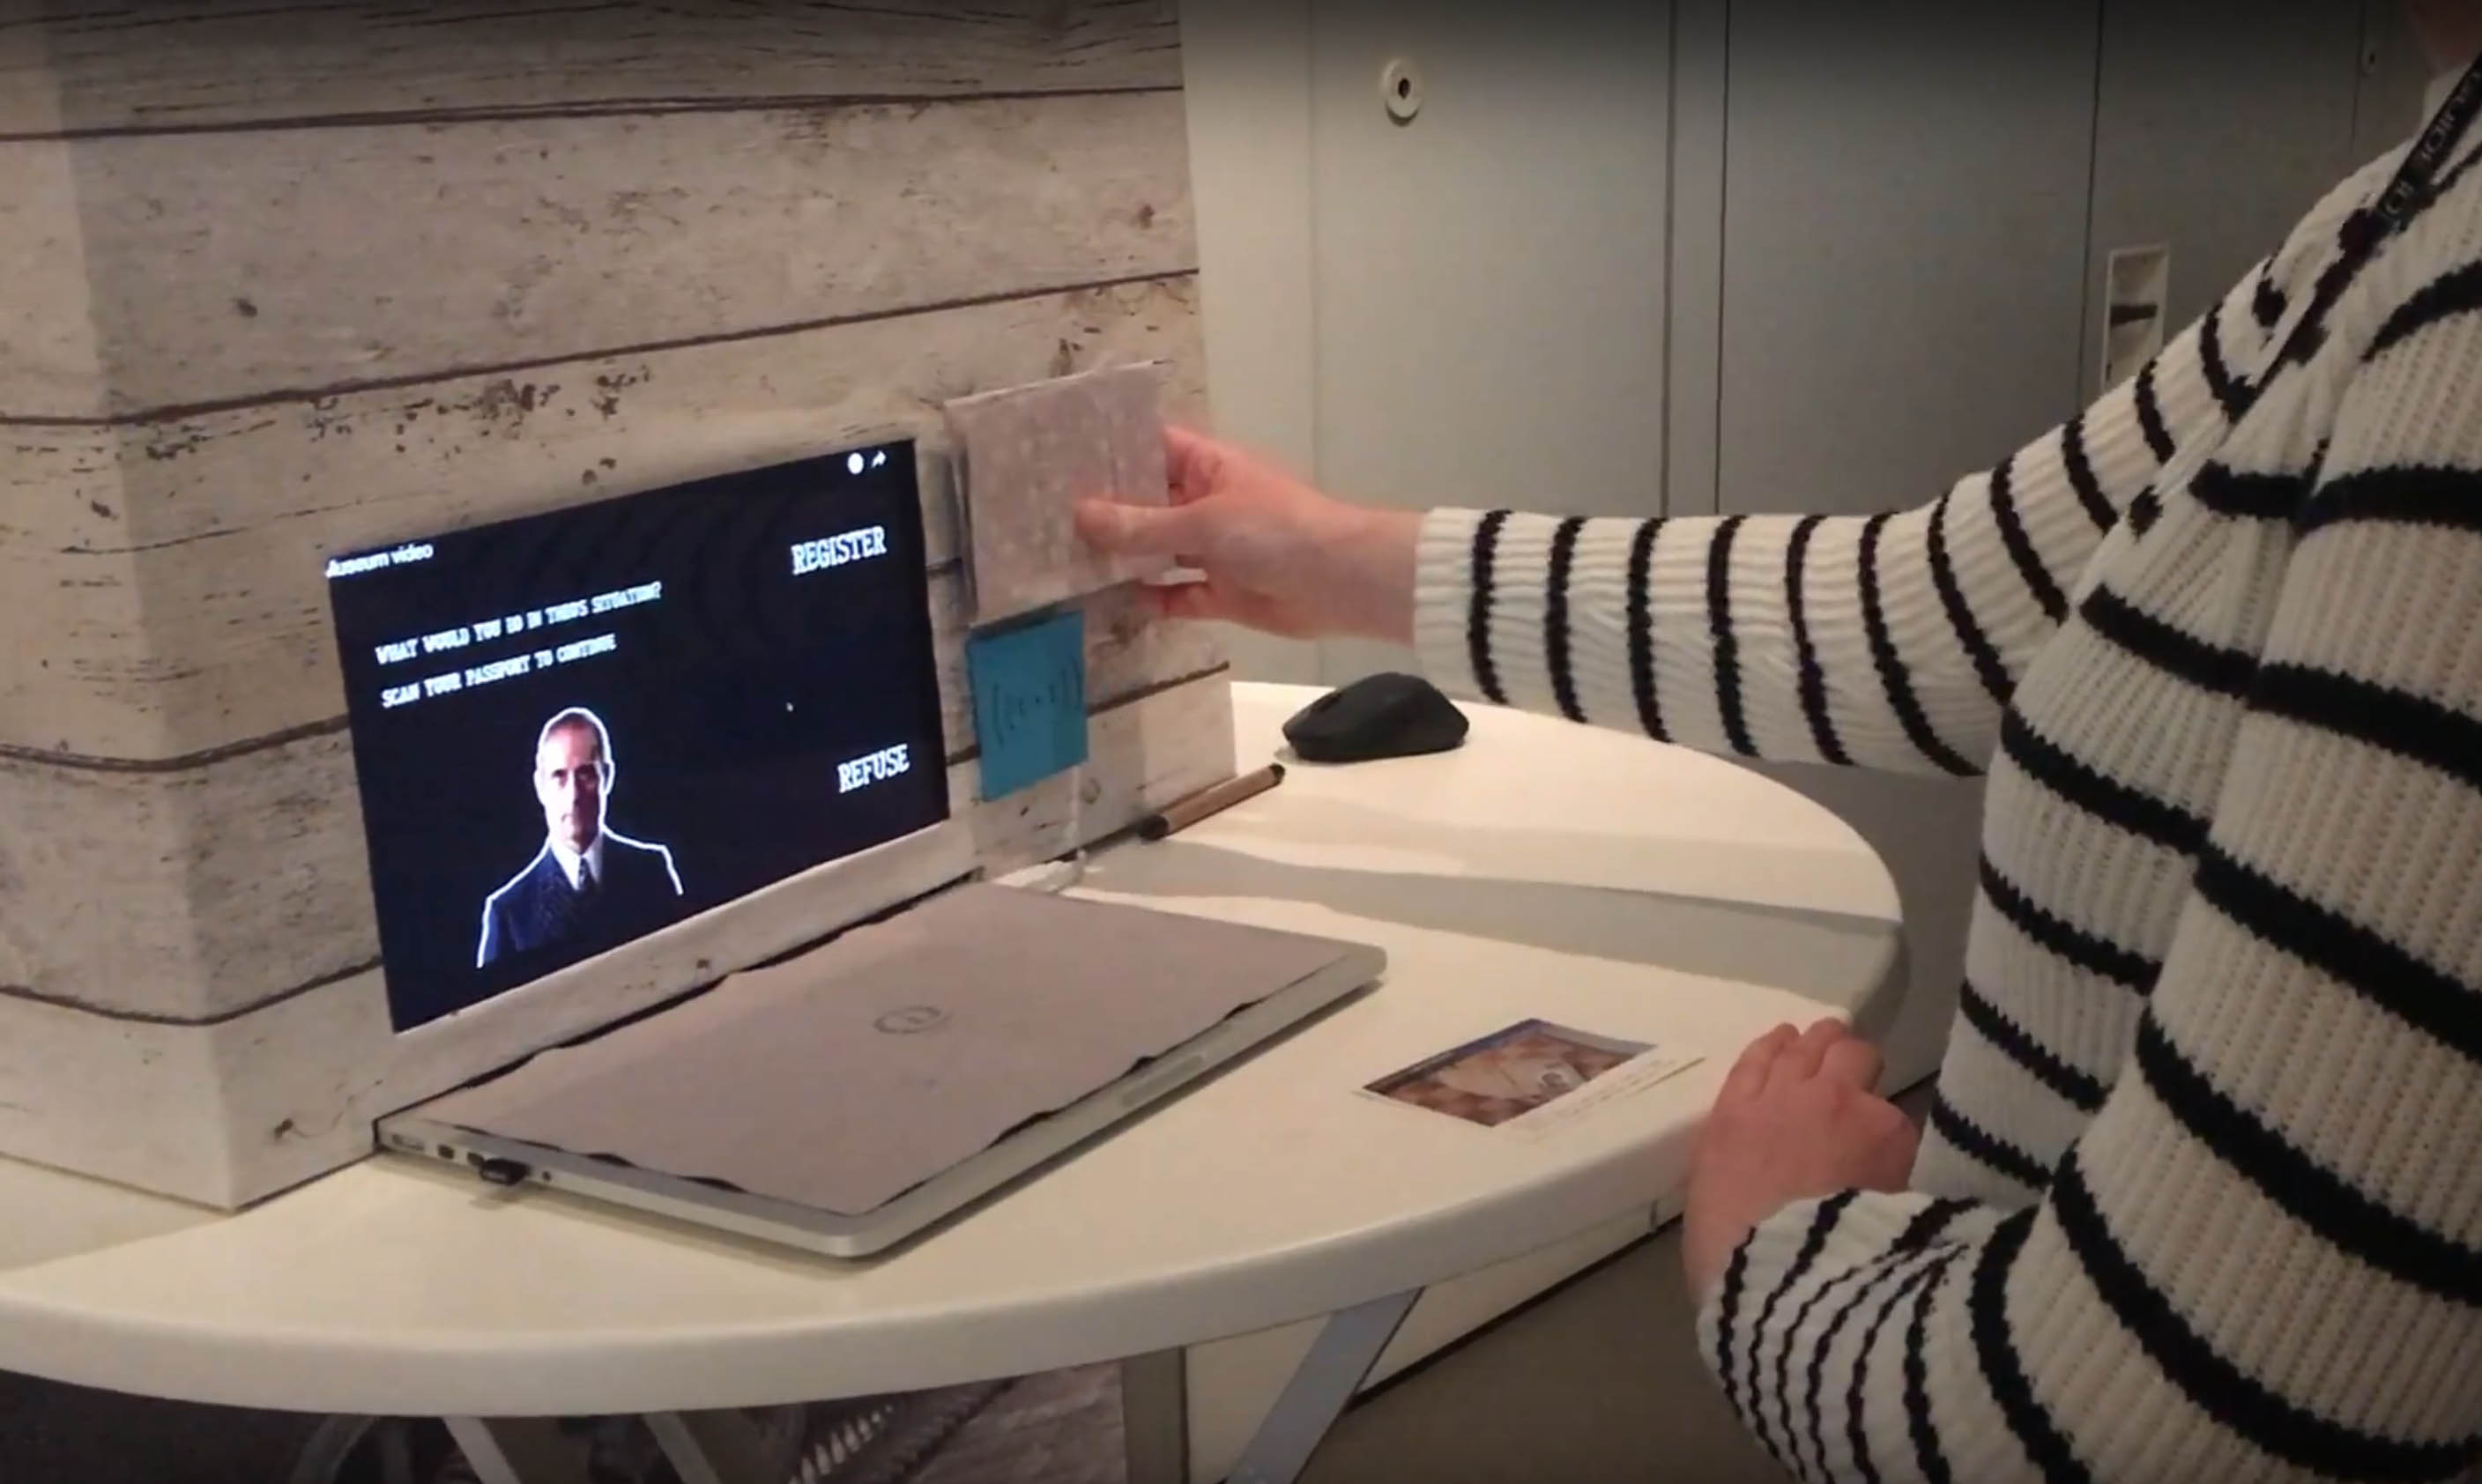
\includegraphics[width=8cm]{assets/test_final1.jpg}
\caption{Functional Prototype Test Session}
\centering
\label{Final_fi}
\end{figure}

The feedback acquired during this final test session revealed that the test participants felt positively connected to the replicated identity card and preferred the animated dilemma station over the textual dilemma station. The test sessions with the groups of two people revealed the need for more encouragement regarding discussion between themselves. Some of the test participants declared that the text speed within the animation was going too fast and suggested the use of voice recordings to make it easier on visitors. The evaluation station was received as very positive and perceived as a good conclusion to the identification rumble experience. However, test participants acknowledged that at the time of testing the evaluation station was relatively empty and that they would envision the station to relate their answers to actual events from the occupation of the Netherlands between 1940 and 1945.


\subsubsection{Final Prototype}
The functional prototype received its final refinements after the final test sessions. This resulted in adding ambient sounds, voice recordings, an encouragement for discussion and a timer of 30 seconds to the animation. The evaluation station now contains more connections to actual events from the time of the occupation and gives visitors more insight into possible consequences of their choices. Lastly, the font used for the text within the animation was adjusted to enhance readability.

\subsection{Final Interaction Journey Proposal} \label{final_int_jour}
\textit{Identification Rumble} is an interactive and engaging experience that integrates new technology into a historical exhibition and creates awareness among visitors regarding dilemmas people faced during the occupation of the Netherlands between 1940 and 1945. Figure \ref{INT_MAP} shows an overview of the museum's main exhibition route with the Identification Rumble interaction points. By using smart replicas of identity cards that were introduced and required in the course of 1941, Identification Rumble facilitates museum visitors of the Dutch Resistance Museum with an experience that is complementary to the historical main exhibition. Moreover, with Identification Rumble visitors engage and connect with the twelve dilemmas to a greater extend and feel more connected to the exhibition and the stories that it tells. 

\begin{figure} [h]
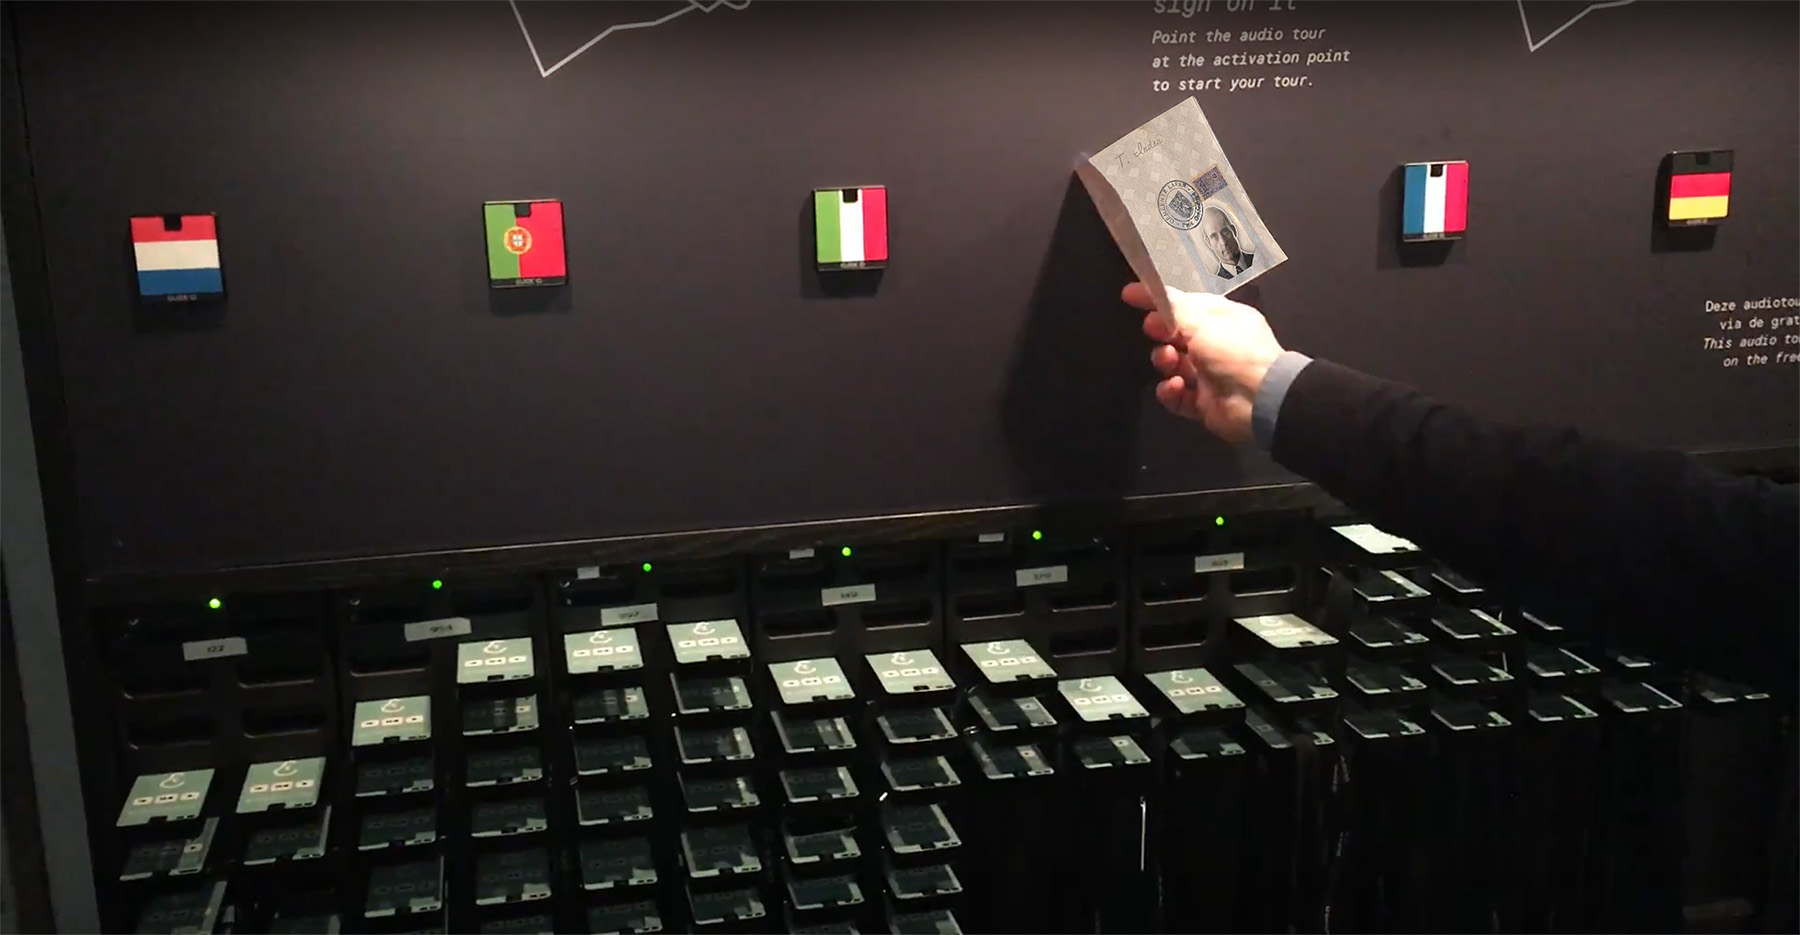
\includegraphics[width=8cm]{assets/lang_pass.jpg}
\caption{Visitors Activate their Identity Card on a Preferred Language Activation Point}
\centering
\label{LANG_PASS}
\end{figure}

\subsubsection{Entrance}
When visitors enter the museum, they first encounter the front-desk where they buy an entrance ticket (Figure \ref{INT_MAP}, point A). With their entrance ticket, visitors also receive a smart replica of a 1940's identity card. The volunteer behind the front-desk informs the visitor that this card is for interacting with certain exhibits. Before entering the exhibition, visitors walk past the language activation wall (Figure \ref{INT_MAP}, point B). On this wall they activate their identity card by holding it against a preferred language activation point (Figure \ref{LANG_PASS}).


\subsubsection{Exhibition Route} Instead of dilemma questions that are projected on the floor, dilemmas are now represented by dilemma stations; interactive exhibits scattered around the exhibition that each uncover a different dilemma. A dilemma station consists of a television screen that is integrated into the wall and two RFID scanners that serve as interaction points. When a visitor approaches a dilemma station the screen shows the message \textit{"Scan your ID Card to start"} accompanied by an arrow that is pointing to a scanner (Figure \ref{SCAN_START}). After the visitor scans their smart replica an animation starts that introduces the dilemma.

The script for the animation is based on real historical events and the characters are depicted using colored pictures of people from WWII (in the prototype the characters are not yet depicted in this way due to time and scope constraints). The choice to realize the animation(s) in this manner is based on the fact that the Dutch Resistance Museum works with real historical imagery to create a story as immersive and realistic as possible.

\begin{figure} [H]
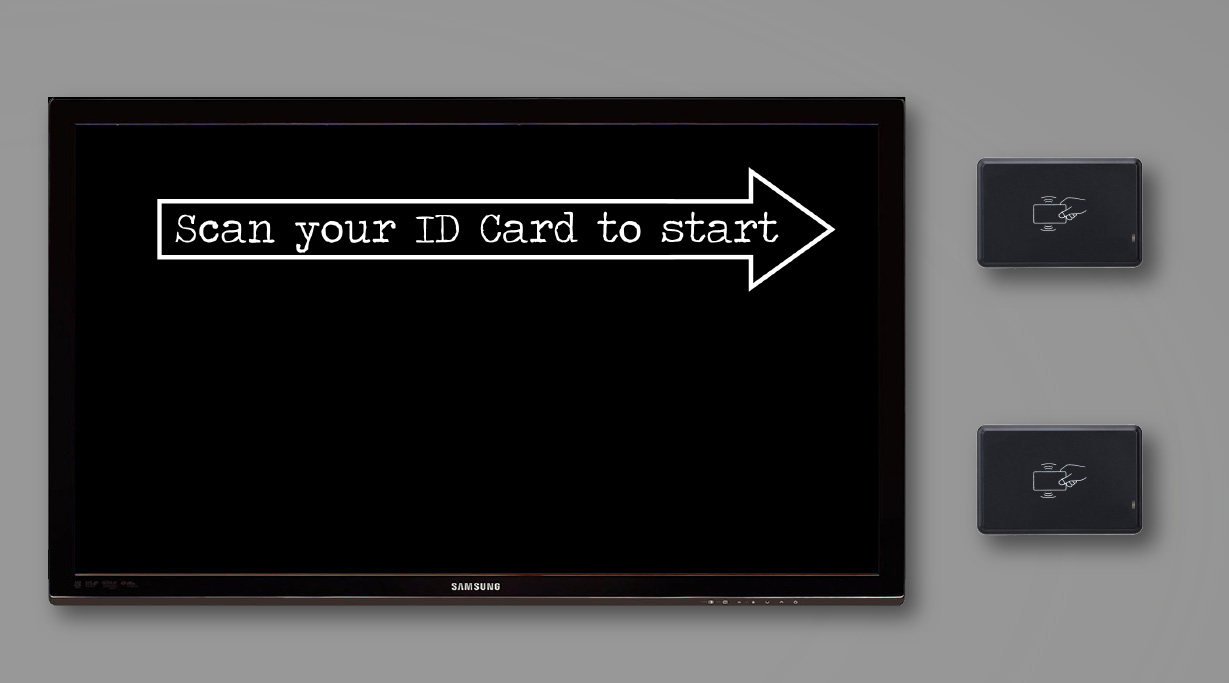
\includegraphics[width=8cm]{assets/scan_start.jpg}
\caption{Dilemma Station Start Screen}
\centering
\label{SCAN_START}
\end{figure}

\subsubsection{Exit}
Approaching the end of the exhibition visitors will find the \textit{Evaluation Station} (Figure \ref{INT_MAP}, point C).
It consists of a television screen and single RFID reader for activation.
In a similar fashion as the dilemma stations, the screen prompts visitors to scan their identity card at the activation point.
Scanning an identity card provides the visitor with an overview split into multiple sections.

The main section, found in the top row, displays a column per dilemma.
These elements state previously made choices in the dilemmas in order to help visitors remembering their journey.
Depending on the answer a visitor has given a real-life consequence is described which people faced during WWII.
This helps to emphasize that there was not necessarily a good choice in these situations.
In addition to that, an individual's choice is compared to previous answers of other visitors.
The comparison indicates whether the answer followed the majority of other people or if it is different.

Remaining space is filled with an overview of visitor language distribution and dynamic sections reserved for changing content.
Showing the language distribution primarily serves the purpose of giving the visitor a feeling who else is visiting the museum.
The dynamic sections can be used by the museum to highlight announcements and incentivize visitors to return their identity card replicas.
Collection points for returned identity cards are positioned next to the evaluation station.

\begin{figure} [H]
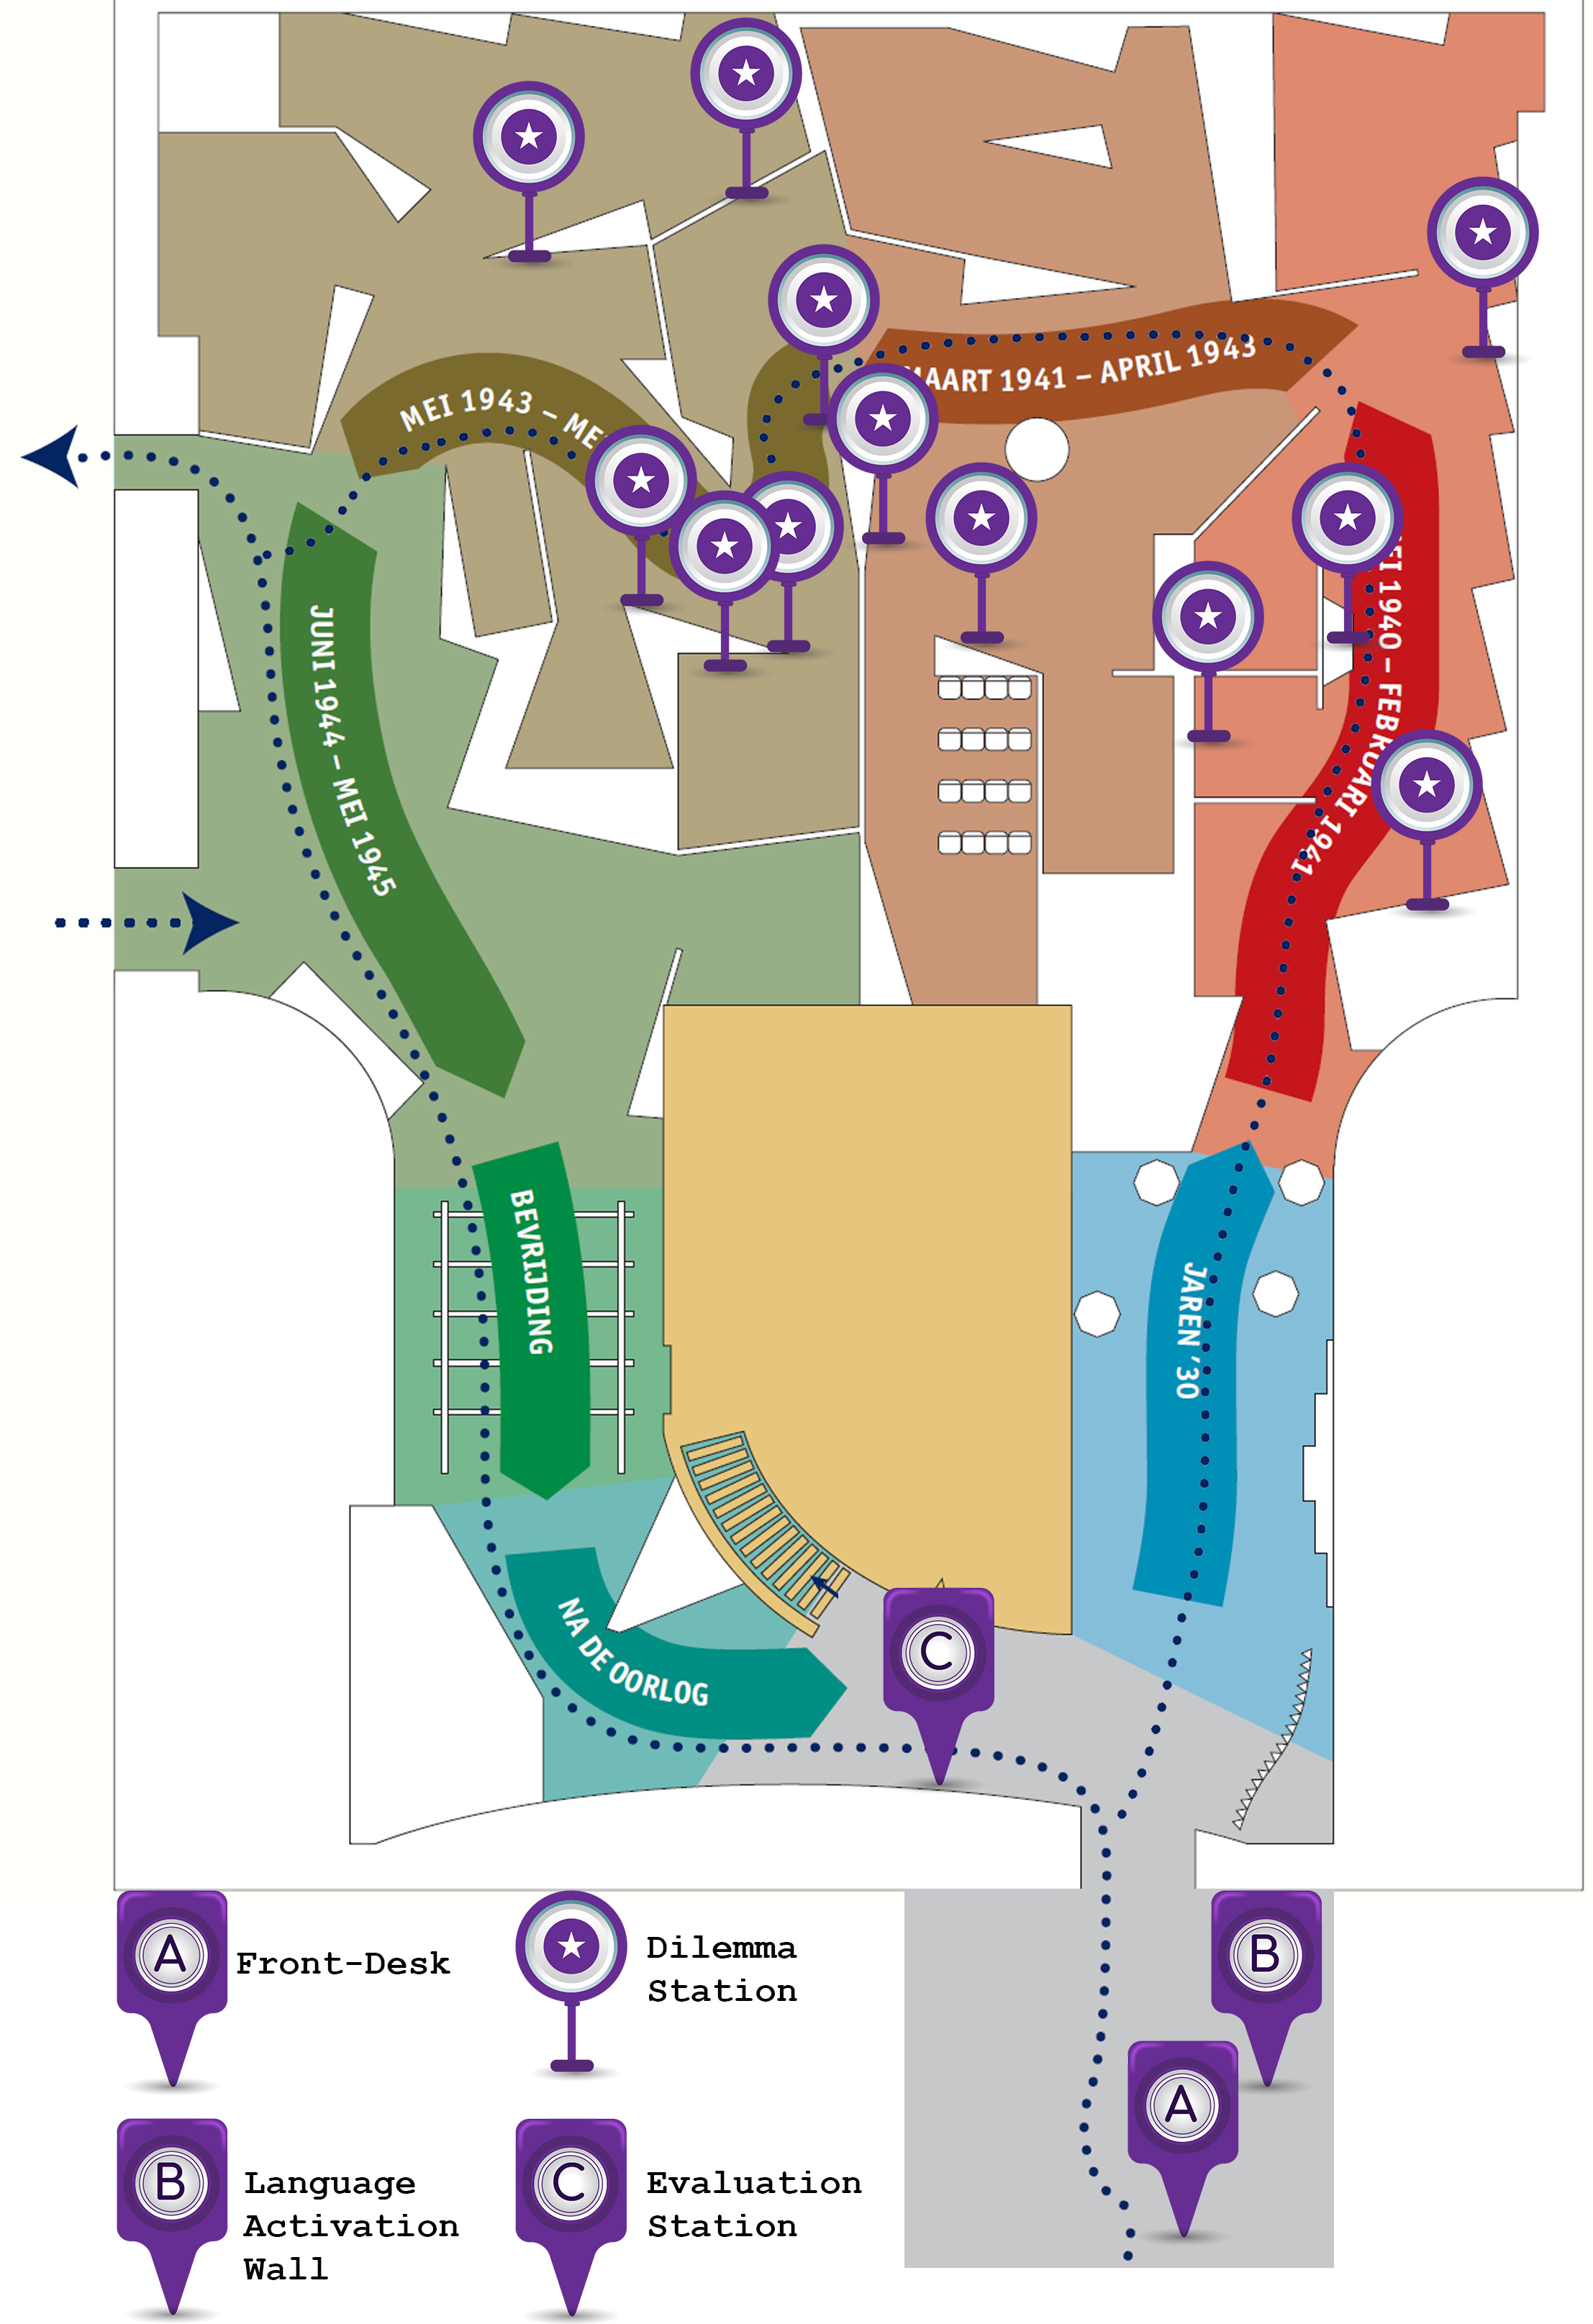
\includegraphics[width=7cm]{assets/Map_Points.jpg}
\caption{Visitor Museum Journey with Interaction Points}
\centering
\label{INT_MAP}
\end{figure}


% !TEX root = ./setup.tex

\section{System Description} \label{System_Description}
Identification Rumble's technical architecture, on a high level, is comprised of the following hardware and software components:

\begin{itemize}
  \item Tangible hardware (identity card replicas)
  \item Static hardware (RFID readers, screens and their connected computer)
  \item Station software (language, dilemma and evaluation station)
  \item Central backend API
\end{itemize}

Software components are realized using web technologies.
JavaScript\footnote{\url{https://developer.mozilla.org/bm/docs/Web/JavaScript}, Accessed: 07-02-2018} is used for front-facing parts of the prototype i.e. stations museum visitors interact with.
This implies that computers used in these stations are capable to run a browser (See Figure \ref{fig:architecture}).
As this project is not a traditionally published website, for visitors using a variety of browsers, no special support has been implemented for edge cases and old browsers.
Instead, the museum is in full control which browsers are deployed.
Currently, recent versions (i.e. last 2) of the following browsers are guaranteed to be supported\footnote{Other browsers and versions can be able to run the prototype as well}:

\begin{itemize}
  \item Google Chrome\footnote{\url{https://www.google.ca/intl/en/chrome/}, Accessed: 07-02-2018}
  \item Mozilla Firefox\footnote{\url{https://www.mozilla.org/en-US/firefox/new}, Accessed: 07-02-2018}
  \item Microsoft Edge\footnote{\url{https://www.microsoft.com/en-us/windows/microsoft-edge}, Accessed: 07-02-2018}
\end{itemize}

Given these constraints, the stakeholder is able to choose any device capable of running these browsers.

The central backend uses Node.js\footnote{\url{https://nodejs.org, Accessed: 07-02-2018}} as its framework and runs TypeScript\footnote{\url{https://www.typescriptlang.org}, Accessed: 07-02-2018} which is a strongly typed superset of JavaScript.
More on this component in section \ref{sec:backend}.

Figure \ref{fig:architecture} visualizes the full system and distinguishes between physical and digital components.
The following sections elaborate on the different parts found in the diagram.
Furthermore, every number corresponds to one of the following sections in ascending order.
This will be made explicit in each section as well.


\subsection{Identity Card Replica} \label{sec:idcardreplica}
Every physical identity card is equipped with an RFID tag inside (Figure \ref{fig:architecture}, marker 1).
These replicas are modeled after the \textit{'persoonsbewijs'} which Dutch citizens were required to carry with them during the German occupation in WWII\footnote{\url{http://www.persoonsbewijzen.nl/} (Dutch), Accessed: 09-02-2018}.
An interactive, visual representation of these identity cards can be found here:

\begin{flushleft}
  \url{https://identification-rumble.science/persoonsbewijs}\footnote{Accessed: 07-02-2018}
\end{flushleft}

Due to the contained RFID tags, these identity cards can be recognized by RFID readers.
Within the range of communication, up to 6cm\footnote{\url{https://www.phidgets.com/?tier=3&catid=81&pcid=72&prodid=23}, Accessed: 07-02-2018}, the scanners are able to read the digital value stored on tags.
With the exception of two tags, the ones used in this prototype are read-only.
Therefore, a simple mapping between the predefined values on the tags to their digital representation can be performed.
Digital identity cards have a unique integer number assigned to them from which they can be retrieved.

\begin{lstlisting}[caption={JavaScript mapping for RFID tags}, label={lst:mapping}, language=JavaScript]
{
  '79001ff8c8': {
    name: 'Card',
    value: 0
  },
  '4a0037db70': {
    name: 'Blue chip',
    value: 1
  },
  ...
}
\end{lstlisting}

In listing \ref{lst:mapping}, a simple JavaScript object uses the RFID tags as its keys.
Each key maps to a descriptive name and a value which represents a unique number of a digital identity card.
The name is merely for administration purposes and helps to identify the physical tag in the mapping interface (See Figure \ref{fig:mappinginterface}).

\begin{figure}[h]
  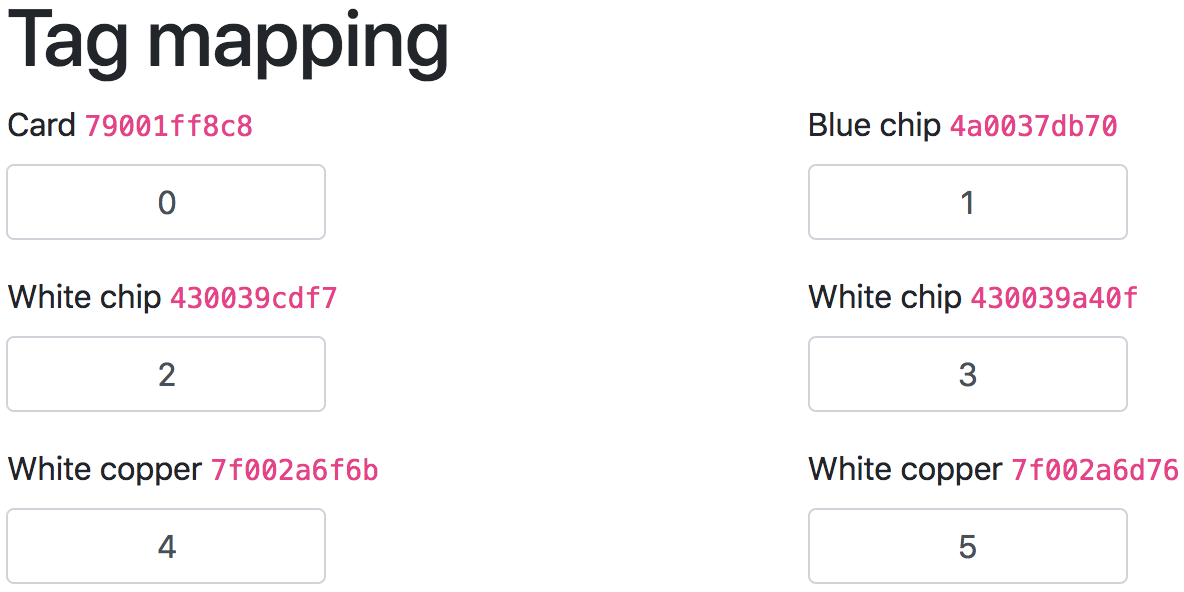
\includegraphics[width=5cm]{assets/mapping-interface.png}
  \caption{Tag mapping interface}
  \centering
  \label{fig:mappinginterface}
\end{figure}


\subsection{Language Scanner}
This station allows visitors to change the language of their experience according to their preference.
Every supported language of the museum is represented by a small physical flag (roughly the size of an identity card).
Each of these flags is equipped with an RFID reader (Figure \ref{fig:architecture}, marker 2).
Upon holding an identity card close to a flag the corresponding tag is recognized.
As previously discussed (Section \ref{sec:idcardreplica}) this tag is then mapped to its corresponding digital identity card.
Finally, the station signals the backend to change the language of this identity card accordingly.
In addition to that, it emits an audible beep noise indicating successful execution.

Changing languages in the prototype is possible at:

\begin{flushleft}
  \url{https://identification-rumble.science/language}\footnote{Accessed: 07-02-2018}
\end{flushleft}


\subsection{Dilemma Station}
Dilemmas require the most hardware in the Identification Rumble prototype.
They consist of a screen, computer and RFID reader for every possible answer.
While the current design only uses two answers, it is possible to provide more choices.
This setup is repeated for every dilemma in the exhibition (Figure \ref{fig:architecture}, marker 3).

In its idle state, the station prompts visitors to hold their identity cards to either of the connected RFID readers.
Scanning the identity card allows the system to retrieve the previously selected language of the visitor.
It continues by playing the corresponding dilemma animation video in the correct language.

Dilemma videos are virtually segmented into three parts:
(1) story, (2) answer prompt and (3) outro.
During the first story segment, the station ignores any recognized identity cards on the RFID readers.
Once it reaches the answer prompt section, scanning an identity card will fast forward the video to the outro.
Finally, the outro provides contextual information to the visitor and concludes the story.
Scanning a different identity card during the outro or after the animation has finished restarts this process.

Answering a dilemma leads to the station sending relevant information to the backend; namely respective IDs of the dilemma, answer and identity card.

This part of the prototype can be found at:

\begin{flushleft}
  \url{https://identification-rumble.science/dilemmas}\footnote{Accessed: 07-02-2018}
\end{flushleft}


\subsection{Evaluation Station} \label{sec:evaluationstation}
The Evaluation Station consists of a screen, RFID reader and computer each (Figure \ref{fig:architecture}, marker 4).
Technically speaking only one station is required to provide the functionality to visitors.
However, depending on the number of visitors trying to access this station at the same time the setup can be repeated.

Scanning an identity card at this station sets it off to fetch two data objects from the backend: (1) selected answers of this identity card and (2) historical statistics of other visitors selected languages and answers.
This information is used to compare personal choices with previous visitors who answered the same.

\begin{lstlisting}[caption={Calculating percentage of visitors who answered the same}, label={lst:samepercentage}, language=JavaScript]
// this.stats.dilemmas: Object<Number, Array<Date>>
const answerStats = this.stats.dilemmas[dilemmaId];
const totalAnswers = Object.values(answerStats).reduce(
    (sum, dates) => sum + dates.length,
    0
);
const sameAnswersCount = answerStats[answerId].length;
const percent = Math.round(
    sameAnswersCount / totalAnswers * 100
);
\end{lstlisting}

In listing \ref{lst:samepercentage}, the percentage comparison is calculated by accessing the answer statistics of an individual dilemma.
Each answer can be inspected by using its ID and contains an array of dates indicating when it was selected.
Counting the total number of dates as well as the number of visitors answering the same allows calculating the final percentage.

Apart from that, two types of charts are shown to visualize answer distribution (vertical bar chart) and the ratio of languages (pie chart).
These charts are realized using the Chartist\footnote{\url{https://gionkunz.github.io/chartist-js/}, Accessed: 08-02-2018} library.

Evaluating choices of an identity card is possible at:

\begin{flushleft}
  \url{https://identification-rumble.science/evaluation}
\end{flushleft}


\subsection{Communication} \label{sec:communication}
Different parts of the system are scattered throughout the exhibition.
In order to trigger actions (language scanner, dilemma station) or fetch information (evaluation station) they have to contact the central backend server.
Therefore, each page starts a bi-directional WebSocket\footnote{\url{https://developer.mozilla.org/en-US/docs/Web/API/WebSocket}, Accessed: 08-02-2018} connection with the server.
As connection loss is not handled by the native WebSocket browser API and to ease usage Socket.IO\footnote{\url{https://socket.io/}, Accessed: 08-02-2018} is used as a library (Figure \ref{fig:architecture}, marker 5).
It provides an event based interface to send data from the client to the server or vice versa.


\subsection{Backend} \label{sec:backend}
The backend API is implemented in TypeScript using Node.js as a framework and runtime (Figure \ref{fig:architecture}, marker 6).
It acts as the central communication unit to which all parts of the system report their changes and can retrieve data.
Responsibility of the backend can be divided into three distinct categories: (1) providing the Socket.IO server (Section \ref{sec:communication}), (2) implementing business logic and (3) persisting state (Section \ref{sec:storage}).

As soon as a client opens a new connection with the Socket.IO server it begins to listen for all possible events.
These events are delegated to their corresponding business logic services.
Table \ref{tbl:eventservices} provides a full overview of event and parameter delegation to services.
While it refers to identity cards the backend code uses the legacy term 'passport' which was used during the conception of the project.

\begin{table}
  \centering
  \begin{tabular}{ |l|l| }
    \hline
    \textbf{Event + Parameters} & \textbf{Service} \\
    \hline
    getPassports() & passport \\
    createPassport() & passport \\
    resetPassport(id) & passport \\
    removePassport(id) & passport \\
    getPassport(id) & passport \\
    changeLanguage(passportId, languageCode) & passport \\
    answerDilemma(passportId, dilemmaId, answerId) & passport \\
    getStats() & statistics \\
    setReadOnlyMode(password, enabled) & settings \\
    getReadOnlyMode() & settings \\
    getTagMapping() & settings \\
    setTagMapping(tag, value) & settings \\
    \hline
  \end{tabular}
  \caption{Delegation of events and parameters to services} \label{tbl:eventservices}
\end{table}


\begin{figure*}
  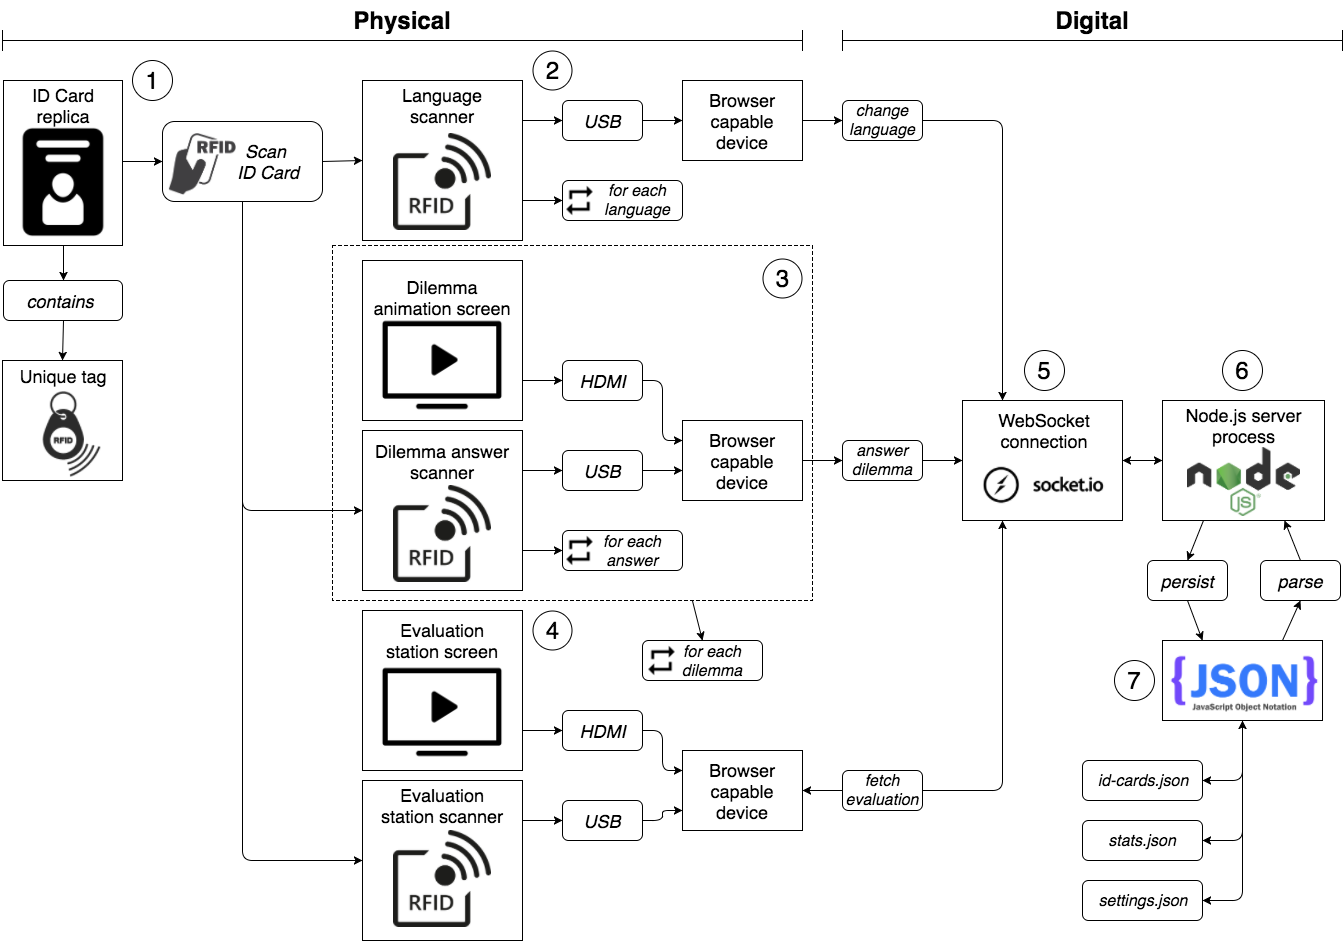
\includegraphics[width=15cm,keepaspectratio]{assets/system-architecture.png}
  \caption{System architecture}
  \label{fig:architecture}
\end{figure*}

The passport service implements a straightforward CRUD\footnote{\url{https://developer.mozilla.org/en-US/docs/Glossary/CRUD}, Accessed: 09-02-2018} (Create, Read, Update, Delete) interface for accessing and manipulating identity cards.
Changing language and answering a dilemma are the two main mutation functions operating on the state of an identity card.
They notify the statistics service of their changes in the background which in turn allow them to provide historical data for the evaluation station (Section \ref{sec:evaluationstation}).

Administrative functionality is handled within the settings service.
It contains a boolean flag indicating whether the system is in a read-only mode disabling creation and deletion of identity cards as well as changes to the tag mapping.
This can be used for presentation purposes or to prevent accidental changes.
Furthermore, the tag mapping discussed in section \ref{sec:idcardreplica} is handled by the settings service.

Restarting the backend should not lead to unexpected data loss.
Therefore, services continuously persist their own state after changes have been made (Section \ref{sec:storage}).


\subsection{Storage} \label{sec:storage}
Persisting state is implemented using plain JSON\footnote{\url{https://www.json.org/}, Accessed: 09-02-2018} (JavaScript Object Notation) files for each service (Figure \ref{fig:architecture}, marker 7).
Before the backend starts to accept connections the services try to parse previous state from these files.
When changes are committed to identity cards, statistics or system settings the respective service triggers an asynchronous write operation of its state.
Executing this operation asynchronously allows the backend to deal with different tasks in the mean time; this is a strong suit of Node.js.

It could be argued that relying on JSON serialization and parsing does not scale well and is inferior to a full blown database system.
While this is true for larger software systems this prototype intentionally avoids database system in spirit of the KISS-principle\footnote{\url{https://people.apache.org/~fhanik/kiss.html}, Accessed: 09-02-2018} (Keep It Simple, Stupid).
KISS is usually applied to code itself but can be adapted to other areas as well, in this case the setup of a software system.
Using a full database system increases the complexity of setup and maintaining the backup.
In addition to that, there is virtually no added value as this system only handles a limited amount of data.
Even with a generous estimate of 100 created identity cards storing their state would still be possible within the constraints of JSON files.
Special query functionality provided by database systems would still not be required as the backend performs lookups in memory.



 \label{systemdescription}

\section{Discussion}

This section provides highlights from the user testing feedback, several limitations to the testing are discussed, recommendations are given on different implementation strategies and both required and optional future work is listed. 

\subsection{User Feedback}
As discussed, user feedback has had a substantial impact on refinements of the prototype. The most important positive feedback includes the positive connection between museum visitors, preferences for animation over text, the replica of the identity card, and the general engagement of the visitors with the dilemmas. 

Most of the received feedback described in section \ref{US_TEST} has been implemented in next iterations of the prototype. Some important feedback that has not been fully implemented in the current prototype includes more encouragement for groups to discuss the answer among themselves, the balance between the text being too fast and the animation being too long, and the visitor's choices have no real world consequences for them. 

\subsection{Limitations}
The presented user tests and methodology include several possible biases. Most importantly, results could be skewed because during user tests, researchers were present to guide test participants through the experience and were asked questions. In its finalized form, this would not be possible. 
Secondly, too few user tests were carried out to provide statistically significant results, though results were highly useful for feedback and ideas for improvements. The implementation of Identification Rumble would require the volunteers of the Dutch Resistance Museum to keep track of additional physical objects, which could be a hindrance for them. User tests in the museum were carried out in the main hall, just in front of the start of the exhibits. This might have influenced user experiences. Also, the prototype is not complete with historically accurate imagery in the animation. The voice over and discussion prompting texts that were added in the final prototype were not subjected to user texts and the final prototype has minor differences in the lay out compared to the lay out the exhibits in their implemented form. 
Finally, the museum could adopt the idea to gift the visitors the identity cards as their production cost is quite low and it might function as a distinct souvenir to take home and remember the museum by. 

\subsection{Conclusion and Recommendation}
Identification Rumble first and foremost provides an interactive experience for visitors. The combination of an animation and the possibility to answer for visitors to give their own answers is engages the visitors to think about the dilemma. This shows a stark contrast to the current exhibits where some visitors do not even notice some dilemmas. Evidently, the implementation of Identification Rumble is recommended. However, this can be done do different extents. 

Firstly, the dilemma does not have to be implemented for every dilemma to make a difference. Current exhibits could gradually be replaced by dilemma stations equipped with RFID readers. However, it is recommended that first implementation should cover at least 5 dilemmas. Otherwise, the role of the evaluation would be far less significant. 

Moreover, the dilemmas do not have to be presented in the same format. For example, dilemmas could differ from each other in terms of duration, interactivity and technology. Also, not all dilemmas necessarily need an animation, though test users did favor animation over plain text. 
Lastly, dilemma stations could be implemented without the RFID system and identity cards entirely and use buttons instead. This does complicate choosing language and eliminates the option for a personal evaluation at the end of the tour. 

\subsection{Future Work}
In order for Identification Rumble to be implemented, some work is still needed. 
To finalize the dilemma \textit{'Register?'}, the animation needs text and voice overs in all the languages used by the Dutch Resistance Museum. 
Also, professional voice overs should be recorded and all copyrighted imagery in the animation must be replaced. 
Furthermore, to extend Identification Rumble to multiple dilemmas, animations are needed as well as historically accurate stories and voice acting in multiple languages. 
In terms of hardware, every dilemma station would also require two RFID readers. 
Then, the language station would require a RFID scanner for every available language, currently six. 
Finally, the evaluation station could reveal personalized stories based on the choices that were made with a single identity card. 

%Fonds21\footnote{\url{https://www.fonds21.nl/}, Accessed: 08-2-2018} and VSBfonds\footnote{\url{https://www.vsbfonds.nl/}, Accessed: 08-2-2018} can be a solution for the money problem. \label{discussion}
\newpage
% !TEX root = ./setup.tex

\section*{Appendix}

\subsection*{Appendix A: Project Homepage}
The project's homepage serves two purposes:
(1) Provide a central information hub for visitors
and (2) host the functional prototype for demonstrations.
It can be reached at:

\begin{flushleft}
  \url{https://identification-rumble.science}
\end{flushleft}

\textbf{Disclaimer:}
The domain \textit{'identification-rumble.science'} has been registered at Namecheap
\footnote{\url{https://namecheap.com}, Accessed: 06-02-2018}
for one year.
At the time of writing it is set to expire on 10th of January 2019.


\subsection*{Appendix B: Source Code}
Development of the project has taken place in a Git
\footnote{\url{https://git-scm.com/}, Accessed: 06-02-2018}
repository hosted on GitHub
\footnote{\url{https://github.com}, Accessed: 06-02-2018}.
It will be indefinitely\footnote{As long as GitHub provides free public repositories.} available at:

\begin{flushleft}
  \url{https://github.com/marc1404/identification-rumble}
\end{flushleft}


\subsection*{Appendix C: Presentation}
On Wednesday, 31st of January 2018 Identification Rumble was presented at AUX'18
\footnote{\url{http://uva-aux.nl/}, Accessed: 06-02-2018}.
The presentation itself consists of slides, a printed poster and a video:

\begin{flushleft}
  \textbf{Presentation:} \break
  \url{https://github.com/marc1404/identification-rumble/blob/master/static/presentation.pdf}
\end{flushleft}

\begin{flushleft}
  \textbf{Poster:} \break
  \url{https://github.com/marc1404/identification-rumble/blob/master/static/poster.pdf}
\end{flushleft}

\begin{flushleft}
  \textbf{Video:} \break
  \url{https://www.youtube.com/watch?v=xYIzAM9P3No}
\end{flushleft}


\subsection*{Appendix D: Forms}
An observation and tally form was used during field trips to the museum.
They were used by the researchers to collect notes in a standardized way.
Participants of usability testing rounds were asked to fill in an informed consent form.
These forms can be found in the GitHub at the following locations:

\begin{flushleft}
  \textbf{Observation form:} \break
  \url{https://github.com/marc1404/identification-rumble/blob/master/static/observation-form.pdf}
\end{flushleft}

\begin{flushleft}
  \textbf{Tally form:} \break
  \url{https://github.com/marc1404/identification-rumble/blob/master/static/tally-form.pdf}
\end{flushleft}

\begin{flushleft}
  \textbf{Informed consent form:} \break
  \url{https://github.com/marc1404/identification-rumble/blob/master/static/informed-consent-form.pdf}
\end{flushleft}

